\documentclass[dvipdfmx]{jlreq}

\usepackage[dvipdfmx]{graphicx}
\usepackage[hidelinks]{hyperref}
\usepackage{float}
\usepackage{svg}
\usepackage{booktabs}
\usepackage{longtable}
\usepackage{array}

% 目次に表示する深さを\subsectionまでに変更
\setcounter{tocdepth}{2}

\begin{document}

\input{sections/title}
\newpage

\tableofcontents
\clearpage

% はじめに
\input{sections/section1_begin.tex}

% システム概要
\section{システム概要}
\subsection{利用者側機能}

\subsubsection{会員機能}
\begin{itemize}   
    \item 新規会員登録
\end{itemize}
一般会員が新規会員登録として,Googleアカウントの情報であるGoogle ID,メールアドレスを
データベースに登録し,会員登録を行う機能.
ログイン画面の「利用規約」をクリックすると,利用規約を表示する.
利用規約に同意する場合,利用規約に同意する旨の項目にチェックし,
「Googleでログイン」を選択すると,Google認証に移る.
Google認証でアカウントを選択すると,Googleによる認証処理が行われる.認証後、
会員情報を格納しているデータベースにアクセスし,選択したGoogleアカウント情報を格納する.
登録後,地図表示画面に遷移する.


\begin{itemize}   
    \item ログイン・ログアウト
\end{itemize}
一般会員がGoogle認証を用いて,任意にログイン・ログアウトを行う機能.

ログイン機能では,ログイン画面の「利用規約」をクリックすると利用規約を表示し,
利用規約に同意する場合,利用規約に同意する旨の項目にチェックし,「Googleでログイン」を選択すると,Google認証に移る.
Google認証でアカウントを選択すると,Googleによる認証処理が行われる.認証後、
会員情報を格納しているデータベースにアクセスし,選択したGoogleアカウント情報がデータベースに
登録済みである場合にログインを許可する.
ログイン後、地図表示画面に遷移する.

ログアウト機能では,すでにログインしている一般会員が任意のタイミングでログアウト操作を行うことができる.
「ログアウト」を選択すると,ログアウト画面に遷移する.ログアウト画面の「キャンセル」を選択した場合,
ログアウト画面へ遷移する前の画面へ遷移する.
「ログアウト」を選択した場合,セッション情報を無効化し,ログイン画面に遷移する.

\begin{itemize}   
    \item 退会
\end{itemize}
一般会員が任意のタイミングで本システムから退会することができる機能.
「マイページ」をクリックし,マイページ画面に遷移する.設定を選択すると「アカウント削除画面へ」
というボタンが表示される.このボタンをクリックすると,退会画面に遷移する.
退会画面では,退会理由(任意)を入力し,削除確認項目にすべてチェックを入れる.
削除確認項目のチェックが不十分な場合,「アカウントを削除する」というボタンにはロックがかかりクリック
することができない.
削除確認項目すべてにチェックを入れ,「キャンセル」を選択した場合,マイページ画面に遷移する.
「アカウントを削除する」を選択した場合,退会確認する旨のメッセージを表示する.
ここで「キャンセル」を選択した場合,退会画面に遷移する.
「OK」を選択した場合,会員情報を格納しているデータベースにアクセスし,会員情報を削除する.
その後,ログイン画面へ遷移する.

\begin{itemize}   
    \item 問い合わせ
\end{itemize}
一般会員が質問や要望をメール形式で運営側に送信することができる機能.
地図表示画面の「お問い合わせ」をクリックすると,お問い合わせ画面に遷移する.
件名・メッセージを入力し,ここで件名・メッセージどちらもまたは片方が未記入の場合,
必須入力が入力されていない旨を表示する.
件名・メッセージ両方入力されている場合は,問い合わせ情報を格納しているデータベースにアクセスし,
問い合わせID,現在の日時,件名,本文(メッセージ),問い合わせユーザーIDを格納する.
その後,「お問い合わせを送信しました。運営からの返信をお待ちください。」と表示する.
運営側からの回答は,一般会員が登録しているGoogleアカウントのメールアドレスへ送信される.

\begin{itemize}   
    \item 事業者申請機能
\end{itemize}
一般会員が事業者会員への昇格を申請するための機能.
地図表示画面の「マイページ」をクリックし,マイページ画面へ遷移する.
マイページ画面に表示される「事業者と登録を申請」を選択すると,事業者登録申請画面へ遷移する.
店舗名の欄に事業者名,電話番号の欄に事業者として使用する電話番号,住所の欄に事業者の住所を
記入した後,「申請」を選択した場合,事業者申請の情報を格納しているデータベースにアクセスし,
申請ID,事業者名,電話番号,住所,申請者ユーザーIDを格納する.
「事業者登録申請を送信しました。運営からの承認をお待ちください。」と表示する.
「申請」を選択せず,「キャンセル」を選択した場合,マイページ画面へ遷移する.


\subsubsection{ピン表示機能}
\begin{itemize}   
    \item 地図上でのピン表示機能
\end{itemize}
他の会員が投稿したピンを地図上に表示する機能.
地図表示画面を表示し,投稿内容を格納しているデータベースにアクセスする.
データベースからマップ上の投稿数を取得し,緯度・経度が同じ地点にある,または「投稿を追加」
から投稿された投稿が50以上の場合,通常のピンの1.3倍の大きさのピンとしてマップ上に描画する.
それ以外の投稿は通常の大きさのピンとしてマップ上に描画される.
また,一般会員による投稿はすべて円形のピンとして描画され,事業者会員による投稿は分に
事業者会員自身が設定したアイコンがピンに描画される.

\begin{itemize}   
    \item ジャンル分け機能
\end{itemize}
投稿時に選択されたジャンルに応じてピンの色を変更する機能.
地図表示画面を表示し,ジャンルの情報を格納しているデータベースにアクセスする.
データベースから表示色を取得し,各ジャンルに割り当てられた固有の色をピンの色に反映する.

\begin{itemize}   
    \item リアクション機能
\end{itemize}
各ピンに対して,他の一般会員がリアクションできる機能.
地図表示画面に描画されたピンを選択しクリックすると,そのピンの投稿内容が表示される.
投稿内容にある「リアクション」を選択すると,投稿内容を格納しているデータベースにアクセスする.
データベースからリアクション数を取得し,「リアクション」を「リアクション済み」に変更,
リアクション数を1足したリアクション数を格納する.
データベースに格納されているリアクション数を反映させる.また,リアクションは匿名で行われる.

\subsubsection{絞り込み機能}
\begin{itemize}   
    \item キーワード検索機能
\end{itemize}
検索窓を使用し,入力したキーワードに応じて情報を検索・絞り込みできる機能.
地図表示画面に表示されている検索窓に検索したいキーワードを入力すると,投稿内容を
格納しているデータベースにアクセスし,データベースの中からキーワードを含む投稿を取得する.
地図表示画面にて、キーワードを含む投稿とピンのみを表示・描画する.投稿は,検索窓の下に
一覧で表示され,ピンは地図上に描画される.

\begin{itemize}   
    \item ジャンル絞り込み機能
\end{itemize}
特定のジャンルに属する投稿・ピンのみを描画する機能.
地図表示画面に表示されているジャンル選択ボタンをクリックし,ジャンルの一覧を表示する.
ジャンルの一覧から任意のジャンルを選択すると,投稿内容とジャンルを格納しているデータベースにアクセスし,
選択されたジャンルの投稿内容を取得し,地図表示画面のジャンル選択ボタンの下に選択したジャンルの投稿のみ
を表示,地図上に選択したジャンルの投稿のピンのみを描画する.

\begin{itemize}   
    \item 期間絞り込み機能
\end{itemize}
指定した日付または期間内に投稿されたピンと投稿のみを表示する機能.
地図表示画面に表示されている期間選択ボタンをクリックし,期間の一覧を表示する.
期間の一覧から任意の期間を選択すると,投稿内容を格納しているデータベースから選択された
期間の投稿内容を取得し,地図表示画面の期間選択ボタンの下に選択した期間の投稿のみが一覧で
表示,地図上に選択した期間の投稿のピンのみを描画する.

\subsubsection{並び替え機能}
\begin{itemize}   
    \item 距離順
\end{itemize}
現在地,または任意の場所から距離の近い順にピンと投稿を並び替えて表示する機能.
地図表示画面に表示されている並び替え選択機能をクリックし,並び替え項目の一覧を表示する.
並び替え項目の一覧から「距離順」を選択すると,投稿内容を格納しているデータベースから投稿内容を
取得し,投稿内容を現在地,または任意の場所から距離の近い順にピンと投稿を並び替える.
地図表示画面の並び替え選択機能の下に並び替えた投稿を表示,地図上には並び替えられた投稿のピン
が描画される.

\begin{itemize}   
    \item リアクション数順
\end{itemize}
リアクションの数が多い順または少ない順にピンと投稿を並び替えて表示する機能.
地図表示画面に表示されている並び替え選択機能をクリックし,並び替え項目の一覧を表示する.
並び替え項目の一覧から「リアクション数順」を選択すると,投稿内容を格納しているデータベースから投稿内容を
取得し,投稿内容をリアクションの数が多い順または少ない順にピンと投稿を並び替える.
地図表示画面の並び替え選択機能の下に並び替えた投稿を表示,地図上には並び替えられた投稿のピン
が描画される.

\begin{itemize}   
    \item 新着順
\end{itemize}
投稿日時が新しい順にピンと投稿を並び替えて表示する機能.
地図表示画面に表示されている並び替え選択機能をクリックし,並び替え項目の一覧を表示する.
並び替え項目の一覧から「新着順」を選択すると,投稿内容を格納しているデータベースから投稿内容を
取得し,投稿内容を投稿日時が新しい順にピンと投稿を並び替える.
地図表示画面の並び替え選択機能の下に並び替えた投稿を表示,地図上には並び替えられた投稿のピン
が描画される.

\subsubsection{ピン投稿機能}
\begin{itemize}   
    \item 場所情報投稿機能
\end{itemize}
一般会員自身がピンとして投稿する機能.
地図表示画面に表示されている「新規投稿」をクリックし,新規投稿画面に遷移する.
新規投稿画面の投稿内容であるタイトル,説明,ジャンル,緯度,経度を入力する.
投稿内容にて写真が任意でアップロードできる.「投稿する」を選択すると,投稿内容を格納している
データベースにアクセスし,投稿内容を格納し,「投稿しました!」という
メッセージを表示する.その後、地図表示画面に遷移し投稿のピンを表示する.
一般会員が投稿した際のピンは共通である.
投稿を取りやめる場合は,新規投稿画面に表示されている「キャンセル」をクリックすると,
地図表示画面に遷移する.

また,新規投稿画面の「投稿内容を入力」の項目について,ピンを表示する位置を入力する必要がある.
位置情報の入力は地図上で選択または,事業者名検索により行う.
位置情報を地図上で選択して入力する場合,新規投稿画面の投稿内容を入力し,「地図上で選択」を選択
すると,地図が表示される.表示された地図の任意の場所をクリックすると,位置情報を取得し,緯度と
経度の項目を入力する.
位置情報を事業者名検索で入力する場合,新規投稿画面の投稿内容を入力し,「事業者名検索」に
事業者名を入力する.事業者会員情報を格納しているデータベースにアクセスし,事業者情報を検索して
入力された事業者名の有無を確認する.検索した事業者名が存在した場合,その事業者の緯度と経度を
入力する.検索した事業者が存在しなかった場合,「その事業者は存在しません」と表示し,新規投稿
画面に遷移する.

\begin{itemize}   
    \item 記述・写真情報投稿機能
\end{itemize}
一般会員自身がつけたピンに対して,説明文等のテキスト,写真情報を投稿できる機能.
地図表示画面に表示されている「新規投稿」をクリックし,新規投稿画面に遷移する.
新規投稿画面の投稿内容で必須入力であるタイトル,説明,緯度,経度を入力する.
必須入力が未記入の場合は、必須入力が未記入である旨を表示する.
任意でジャンルを選択,また写真をアップロードできる.
必須入力がすべて入力されていた場合,投稿内容を格納しているデータベースにアクセスし,
投稿内容を格納する.その後、「投稿しました!」と表示する.

\begin{itemize}   
    \item 時間情報登録機能
\end{itemize}
一般会員がピンの投稿,記述・写真を投稿した際の日時を登録する機能.
新規投稿画面に表示されている「投稿する」を選択したとき,現在日時を取得し,
投稿内容を格納しているデータベースにアクセスし,投稿した日時をデータベースに格納する.

\begin{itemize}   
    \item ジャンル登録機能
\end{itemize}
一般会員が投稿内容のジャンルを登録できる機能.
地図表示画面に表示されている「新規投稿」をクリックし,新規投稿画面に遷移する.
新規投稿画面のジャンル選択ボタンを選択し,ジャンルの項目を展開して表示する.
展開されたジャンルの項目の中から任意のジャンルを選択し,新規投稿画面のその他の必須入力
を入力した上で「投稿する」を選択する.投稿内容を格納しているデータベースにアクセスし,ジャンル
を格納する.また,ジャンルのデフォルトは「その他」となっている.

\begin{itemize}   
    \item 投稿追加機能
\end{itemize}
一般会員がすでに存在しているピンに対して,投稿を追加できる機能.
地図表示画面に表示されている任意のピンを選択すると,そのピンの投稿閲覧画面に遷移する.
「投稿を追加」を選択すると,新規投稿画面に遷移する.
新規投稿画面の必須入力であるタイトル,説明,緯度,経度を入力し,また必須入力が未記入の場合は
必須入力が未記入である旨を表示する.
必須入力を入力し,「投稿する」を選択すると,投稿内容を格納しているデータベースにアクセスし,
投稿内容を格納する.その際に、ピンに対する投稿数を1増やす.ピンに対する投稿数が50以上ならば
ピンの大きさを通常の1.3倍の大きさにして地図表示画面の地図上に表示するようにする.
ピンに対する投稿数が50未満の場合は,ピンの大きさは通常の大きさで地図表示画面の地図上に表示
する.

\subsubsection{マイページ機能}
\begin{itemize}   
    \item リアクション履歴閲覧機能
\end{itemize}
一般会員自身がこれまでにリアクションを行った投稿の履歴を閲覧できる機能.
「マイページ」を選択すると,マイページ画面に遷移する.
マイページ画面のタブ内にある「リアクション履歴」を選択すると,リアクションの情報を格納している
データベースにアクセスし,リアクションを取得することで,一般会員自身のリアクション履歴を表示する.

\begin{itemize}   
    \item 投稿履歴閲覧機能
\end{itemize}
一般会員自身がこれまでに投稿したピン投稿の履歴を一覧で確認できる機能.
「マイページ」を選択すると,マイページ画面に遷移する.
マイページ画面のタブ内にある「投稿履歴」を選択すると,投稿内容を格納しているデータベースにアクセスし,
投稿内容を取得することで,一般会員自身の投稿履歴を表示する.

\begin{itemize}   
    \item 投稿内容削除機能
\end{itemize}
一般会員自身がこれまでに投稿したものを削除できる機能.
「マイページ」を選択すると,マイページ画面に遷移する.
マイページ画面のタブ内にある「投稿履歴」を選択すると,投稿内容を格納しているデータベースにアクセスし,
投稿内容を取得することで,一般会員自身の投稿履歴を表示する.
表示された投稿履歴の任意の投稿の横にあるゴミ箱マークを選択すると,投稿削除を確認する旨が表示される.
「キャンセル」を選択した場合,マイページ画面に遷移する.「OK」を選択した場合,
投稿内容を格納しているデータベースにアクセスし,任意の投稿内容を削除する.
その後,「投稿を削除しました」と表示する.

\subsubsection{通報機能}
一般会員が不適切な投稿を運営へ通知するための機能.
投稿閲覧画面で「通報」を選択すると,通報理由の入力フォームが表示され,通報理由を入力する.
「通報する」を選択したとき,通報理由が入力されていない場合,通報理由が入力されていない旨を表示し、
通報理由の入力フォームが表示される.通報理由が入力されていた場合,投稿内容の通報の情報を格納する
データベースにアクセスし,通報ID,通報したユーザーのユーザーID,対象投稿ID, 通報理由,通報日時を
格納する.その後,「通報を受け付けました。運営が確認いたします。」と表示する.

\subsubsection{ブロック機能}
\begin{itemize}   
    \item ブロック機能
\end{itemize}
一般会員が特定の利用者に対して表示制限を行うための機能.
投稿閲覧画面の「ブロック」を選択すると,「このユーザーをブロックしますか?ブロックする
と相手の投稿が表示されなくなります。」と表示される.「キャンセル」を選択した場合,
投稿閲覧画面に遷移する.「OK」を選択した場合,会員情報を格納しているデータベースから該当の会員情報
を取得し,またブロックの情報を格納しているデータベースに取得した会員情報をブロック情報として格納する.
その後,「ユーザーをブロックしました」と表示し,地図表示画面に遷移する.

\begin{itemize}   
    \item ブロック解除機能
\end{itemize}
一般会員が特定の利用者に対して表示制限を行う機能.
マイページ画面の設定のタブをクリックすると,ブロックリストが表示される.
任意のユーザーの「ブロック解除」を選択すると,ブロックの情報を格納したデータベースにアクセスし,
任意のユーザーIDを削除する.その後,ブロックリストからユーザーIDを消去する.



\subsection{事業者側機能}

\subsubsection{会員機能}
\begin{itemize}
    \item ログイン・ログアウト
\end{itemize}
事業者会員がGoogle認証を用いて,任意にログイン・ログアウトを行う機能.

ログイン機能では,ログイン画面の「利用規約」をクリックすると利用規約を表示し,
利用規約に同意する場合,利用規約に同意する旨の項目にチェックし,「Googleでログイン」を選択すると,Google認証に移る.
Google認証でアカウントを選択すると,Googleによる認証処理が行われる.認証後,
会員情報を格納しているデータベースにアクセスし,選択したGoogleアカウント情報がデータベースに
登録済みである場合にログインを許可する.
ログイン後,地図表示画面に遷移する.

ログアウト機能では,すでにログインしている事業者会員が任意のタイミングでログアウト操作を行うことができる.
「ログアウト」を選択すると,ログアウト画面に遷移する.ログアウト画面の「キャンセル」を選択した場合,
ログアウト画面へ遷移する前の画面へ遷移する.
「ログアウト」を選択した場合,セッション情報を無効化し,ログイン画面に遷移する.

\begin{itemize}
    \item 退会
\end{itemize}
事業者会員が任意のタイミングで本システムから退会することができる機能.
「マイページ」をクリックし,マイページ画面に遷移する.設定を選択すると「アカウント削除画面へ」
というボタンが表示される.このボタンをクリックすると,退会画面に遷移する.
退会画面では,退会理由(任意)を入力し,削除確認項目にすべてチェックを入れる.
削除確認項目のチェックが不十分な場合,「アカウントを削除する」というボタンにはロックがかかりクリック
することができない.
削除確認項目すべてにチェックを入れ,「キャンセル」を選択した場合,マイページ画面に遷移する.
「アカウントを削除する」を選択した場合,退会確認する旨のメッセージを表示する.
ここで「キャンセル」を選択した場合,退会画面に遷移する.
「OK」を選択した場合,会員情報を格納しているデータベースにアクセスし,会員情報を削除する.
その後,ログイン画面へ遷移する.

\begin{itemize}
    \item 問い合わせ
\end{itemize}
事業者会員が質問や要望をメール形式で運営側に送信することができる機能.
地図表示画面の「お問い合わせ」をクリックすると,お問い合わせ画面に遷移する.
件名・メッセージを入力し,ここで件名・メッセージどちらもまたは片方が未記入の場合,
必須入力が入力されていない旨を表示する.
件名・メッセージ両方入力されている場合は,問い合わせ情報を格納しているデータベースにアクセスし,
問い合わせID,現在の日時,件名,本文(メッセージ),問い合わせユーザーIDを格納する.
その後,「お問い合わせを送信しました。運営からの返信をお待ちください。」と表示する.
運営側からの回答は,一般会員が登録しているGoogleアカウントのメールアドレスへ送信される.

\subsubsection{ピン表示機能}
\begin{itemize}
    \item 地図上でのピン表示機能
\end{itemize}
他の会員が投稿したピンを地図上に表示する機能.
地図表示画面を表示し,投稿内容を格納しているデータベースにアクセスする.
データベースからマップ上の投稿数を取得し,緯度・経度が同じ地点にある,または「投稿を追加」
から投稿された投稿が50以上の場合,通常のピンの1.3倍の大きさのピンとしてマップ上に描画する.
それ以外の投稿は通常の大きさのピンとしてマップ上に描画される.
また,一般会員による投稿はすべて円形のピンとして描画され,事業者会員による投稿は
事業者会員自身が設定したアイコンがピンに描画される.

\begin{itemize}
    \item ジャンル分け機能
\end{itemize}
投稿時に選択されたジャンルに応じてピンの色を変更する機能.
地図表示画面を表示し,ジャンルの情報を格納しているデータベースにアクセスする.
データベースから表示色を取得し,各ジャンルに割り当てられた固有の色をピンの色に反映する.

\subsubsection{ピン投稿機能}
\begin{itemize}
    \item 場所情報投稿機能
\end{itemize}
事業者会員自身がピンとして投稿する機能.
地図表示画面に表示されている「新規投稿」をクリックし,新規投稿画面に遷移する.
新規投稿画面の投稿内容であるタイトル,説明,ジャンル,緯度,経度を入力する.
投稿内容にて写真が任意でアップロードできる.「投稿する」を選択すると,投稿内容を格納している
データベースにアクセスし,投稿内容を格納し,「投稿しました!」という
メッセージを表示する.その後,地図表示画面に遷移し投稿のピンを表示する.
一般会員が投稿した際のピンは共通である.
投稿を取りやめる場合は,新規投稿画面に表示されている「キャンセル」をクリックすると,
地図表示画面に遷移する.

また,新規投稿画面の「投稿内容を入力」の項目について,ピンを表示する位置を入力する必要がある.
位置情報の入力は地図上で選択または,事業者名検索により行う.
位置情報を地図上で選択して入力する場合,新規投稿画面の投稿内容を入力し,「地図上で選択」を選択
すると,地図が表示される.表示された地図の任意の場所をクリックすると,位置情報を取得し,緯度と
経度の項目を入力する.
位置情報を事業者名検索で入力する場合,新規投稿画面の投稿内容を入力し,「事業者名検索」に
事業者名を入力する.事業者会員情報を格納しているデータベースにアクセスし,事業者情報を検索して
入力された事業者名の有無を確認する.検索した事業者名が存在した場合,その事業者の緯度と経度を
入力する.検索した事業者が存在しなかった場合,「その事業者は存在しません」と表示し,新規投稿
画面に遷移する.

\begin{itemize}
    \item 記述・写真情報投稿機能
\end{itemize}
事業者会員自身がつけたピンに対して,説明文等のテキスト,写真情報を投稿できる機能.
地図表示画面に表示されている「新規投稿」をクリックし,新規投稿画面に遷移する.
新規投稿画面の投稿内容で必須入力であるタイトル,説明,緯度,経度を入力する.
必須入力が未記入の場合は,必須入力が未記入である旨を表示する.
任意でジャンルを選択,また写真をアップロードできる.
必須入力がすべて入力されていた場合,投稿内容を格納しているデータベースにアクセスし,
投稿内容を格納する.その後,「投稿しました!」と表示する.

\begin{itemize}
    \item 時間情報登録機能
\end{itemize}
事業者会員がピンの投稿,記述・写真を投稿した際の日時を登録する機能.
新規投稿画面に表示されている「投稿する」を選択したとき,現在日時を取得し,
投稿内容を格納しているデータベースにアクセスし,投稿した日時をデータベースに格納する.

\begin{itemize}
    \item ジャンル登録機能
\end{itemize} 
事業者会員が投稿内容のジャンルを登録できる機能.
地図表示画面に表示されている「新規投稿」をクリックし,新規投稿画面に遷移する.
新規投稿画面のジャンル選択ボタンを選択し,ジャンルの項目を展開して表示する.
展開されたジャンルの項目の中から任意のジャンルを選択し,新規投稿画面のその他の必須入力
を入力した上で「投稿する」を選択する.投稿内容を格納しているデータベースにアクセスし,ジャンル
を格納する.また,ジャンルのデフォルトは「その他」となっている.

\begin{itemize}
    \item 投稿追加機能
\end{itemize}
事業者会員がすでに存在しているピンに対して,投稿を追加できる機能.
地図表示画面に表示されている任意のピンを選択すると,そのピンの投稿閲覧画面に遷移する.
「投稿を追加」を選択すると,新規投稿画面に遷移する.
新規投稿画面の必須入力であるタイトル,説明,緯度,経度を入力し,また必須入力が未記入の場合は
必須入力が未記入である旨を表示する.
必須入力を入力し,「投稿する」を選択すると,投稿内容を格納しているデータベースにアクセスし,
投稿内容を格納する.その際に,ピンに対する投稿数を1増やす.ピンに対する投稿数が50以上ならば
ピンの大きさを通常の1.3倍の大きさにして地図表示画面の地図上に表示するようにする.
ピンに対する投稿数が50未満の場合は,ピンの大きさは通常の大きさで地図表示画面の地図上に表示
する.

\subsubsection{マイページ機能}
\begin{itemize}
    \item 投稿履歴閲覧機能
\end{itemize}
事業者会員自身がこれまでに投稿したピン投稿の履歴を一覧で確認できる機能.
「マイページ」を選択すると,マイページ画面に遷移する.
マイページ画面のタブ内にある「投稿履歴」を選択すると,投稿内容を格納しているデータベースにアクセスし,
投稿内容を取得することで,事業者会員自身の投稿履歴を表示する.

\begin{itemize}
    \item 投稿内容削除機能
\end{itemize}
事業者会員自身がこれまでに投稿したものを削除できる機能.
「マイページ」を選択すると,マイページ画面に遷移する.
マイページ画面のタブ内にある「投稿履歴」を選択すると,投稿内容を格納しているデータベースにアクセスし,
投稿内容を取得することで,事業者会員自身の投稿履歴を表示する.
表示された投稿履歴の任意の投稿の横にあるゴミ箱マークを選択すると,投稿削除を確認する旨が表示される.
「キャンセル」を選択した場合,マイページ画面に遷移する.「OK」を選択した場合,
投稿内容を格納しているデータベースにアクセスし,任意の投稿内容を削除する.
その後,「投稿を削除しました」と表示する.

\begin{itemize}
    \item ダッシュボード機能
\end{itemize}
事業者会員自身がこれまでの投稿に対するリアクション数の推移や閲覧数を閲覧できる機能.
「ダッシュボード」を選択すると,ダッシュボード画面に遷移する.
ダッシュボード画面の「概要」を選択すると,投稿内容を格納しているデータベースにアクセスし,事業者会員自身がこれまで投稿した全ての投稿
のジャンル,リアクション数,閲覧数を取得することで,総投稿数,総リアクション数,総閲覧数,
エンゲージメント率,週間推移,人気投稿を算出し表示する.

\begin{itemize}
    \item 支払い状況確認機能
\end{itemize}
事業者会員自身の現在の契約状況や支払い履歴,次回の請求日・支払額が確認できる機能.
「ダッシュボード」を選択すると,ダッシュボード画面に遷移する.
ダッシュボード画面の「支払い情報」を選択すると,事業者会員情報の支払いの情報を格納している
データベースにアクセスし,支払額,支払日を取得することで,プラン名,料金,次回請求日,支払い履歴
を表示する.

\subsubsection{通報機能}
事業者会員が不適切な投稿を運営へ通知するための機能.
投稿閲覧画面で「通報」を選択すると,通報理由の入力フォームが表示され,通報理由を入力する.
「通報する」を選択したとき,通報理由が入力されていない場合,通報理由が入力されていない旨を表示し,
通報理由の入力フォームが表示される.通報理由が入力されていた場合,投稿内容の通報の情報を格納する
データベースにアクセスし,通報ID,通報したユーザーのユーザーID,対象投稿ID, 通報理由,通報日時を
格納する.その後,「通報を受け付けました。運営が確認いたします。」と表示する.

\subsubsection{ブロック機能}
\begin{itemize}
    \item ブロック機能
\end{itemize}
事業者会員が特定の利用者に対して表示制限を行うための機能.
投稿閲覧画面の「ブロック」を選択すると,「このユーザーをブロックしますか?ブロックする
と相手の投稿が表示されなくなります。」と表示される.「キャンセル」を選択した場合,
投稿閲覧画面に遷移する.「OK」を選択した場合,会員情報を格納しているデータベースから該当の会員情報
を取得し,またブロックの情報を格納しているデータベースに取得した会員情報をブロック情報として格納する.
その後,「ユーザーをブロックしました」と表示し,地図表示画面に遷移する.

\begin{itemize}
    \item ブロック解除機能
\end{itemize}
事業者会員が特定の利用者に対して表示制限を行う機能.
マイページ画面の設定のタブをクリックすると,ブロックリストが表示される.
任意のユーザーの「ブロック解除」を選択すると,ブロックの情報を格納したデータベースにアクセスし,
任意のユーザーIDを削除する.その後,ブロックリストからユーザーIDを消去する.
\subsection{管理者側機能}
\subsubsection{ログイン・ログアウト機能}
管理者がGoogle認証を用いて,任意にログイン・ログアウトを行う機能.

ログイン機能では,ログイン画面の「利用規約」をクリックすると利用規約を表示し,
利用規約に同意する場合,利用規約に同意する旨の項目にチェックし,「Googleでログイン」を選択すると,Google認証に移る.
Google認証でアカウントを選択すると,Googleによる認証処理が行われる.認証後、
会員情報を格納しているデータベースにアクセスし,選択したGoogleアカウント情報がデータベースに
登録済みである場合にログインを許可する.
ログイン後、地図表示画面に遷移する.

ログアウト機能では,すでにログインしている一般会員が任意のタイミングでログアウト操作を行うことができる.
「ログアウト」を選択すると,ログアウト画面に遷移する.ログアウト画面の「キャンセル」を選択した場合,
ログアウト画面へ遷移する前の画面へ遷移する.
「ログアウト」を選択した場合,セッション情報を無効化し,ログイン画面に遷移する.

\subsubsection{投稿削除機能}
管理者が本サービスを利用しているユーザーの投稿を削除することができる機能.
投稿管理タブを選択すると,投稿内容を格納しているデータベースにアクセスし,投稿内容を取得することで,
投稿管理画面に投稿を一覧で表示し,投稿管理画面に遷移する.
投稿管理画面に表示されている投稿一覧の中から任意の投稿の右に表示されているゴミ箱マークをクリック
することで,投稿内容を格納したデータベースにアクセスし,該当の投稿を削除する.
その後、「削除しました」と表示される.


\subsubsection{アカウント削除機能}
管理者が本サービスを利用しているユーザーのアカウントを削除することができる機能.
ユーザー管理タブを選択すると,会員情報を格納しているデータベースにアクセスし,遷移した
ユーザー管理画面にユーザー一覧を表示する.ユーザー管理画面に表示されているユーザー一覧の中から
任意のユーザーの欄の右に表示されているゴミ箱マークをクリックすることで,会員情報を格納している
データベースにアクセスし,該当のユーザーの会員情報をデータベースから削除する.
その後,「削除しました!」と表示する.

\subsubsection{事業者アカウントへの変更機能}


\subsubsection{問い合わせへの対応機能}

\subsubsection{運用状況モニタリング機能}


% コーディング規約
\section{コーディング規約}
以下に本プロジェクトで採用するコーディング規約を示す.



\subsection{HTML}
以下に本システムに用いられたHTMLファイルに適用されるコーディング規約を示す.

\subsubsection{命名規約}
\begin{itemize}
    \item ファイル名
    \begin{itemize}
        \item アッパーキャメルケース(例:CamelCase)表記を使用する
        \item シンプルで内容を示す英単語で構成する
    \end{itemize}    
\end{itemize}

\subsubsection{ドキュメント構造}
全てのHTMLファイルは以下の構造に従う.

\begin{verbatim}
<!DOCTYPE html>
<html lang="ja">
    <head>
        <meta charset="utf-8" />
        <meta name="viewport" content="width=device-width, initial-scale=1.0" />
        <title>ページのタイトル</title>
        <link rel="stylesheet" href="styles.css" />
    </head>
    <body>
        <!-- ページのコンテンツ -->

        <script src="main.js"></script>
    </body>
</html>
\end{verbatim}

    \begin{itemize}
        \item DOCTYPE 宣言を行う.
        \item コメントアウトは「\verb|<!-- コメントアウト -->」で書く
        
    \end{itemize}



\subsection{CSS}
以下に本システムに用いられたCSSファイルに適用されるコーディング規約を示す.

\subsubsection{命名規約}
\begin{itemize}
    \item クラス名
    \begin{itemize}
        \item 役割が分かるように命名する
        \item ケバブケース(小文字,ハイフン)表記を使用する
    \end{itemize}  
\end{itemize}  

\subsubsection{インデント}
\begin{itemize}
        \item タブの使用は禁止する
        \item スペース2つで対応する
\end{itemize} 

\subsubsection{コメント規約}
\begin{itemize}
  \item セクションコメント
    \begin{itemize}
        \item ブロックコメントでセクション名を明記する
        \item 上下に装飾線を入れる
   \end{itemize}  
  \item 行コメント
   \begin{itemize}
    \item ブロックコメントで補足などを書く
   \end{itemize}
\end{itemize}
  
  





\subsection{Go}
以下に本システムに用いられたGoファイルに適用されるコーディング規約を示す.

\subsubsection{命名規約}
\begin{itemize}
    \item パッケージ名
    \begin{itemize}
        \item 小文字の単語で簡潔に表記する
    \end{itemize}  
    \item 関数名・構造体
    \begin{itemize}
       \item 外部に公開する場合,先頭を大文字にする
       \item アッパーキャメルケースとキャメルケースを使い分ける
       \item アンダースコアは使用しない
    \end{itemize}  
    \item インターフェース名
    \begin{itemize}
        \item 単一メソッドインターフェースは-er接尾辞を使用する
    \end{itemize}  
      
\end{itemize}

\subsubsection{インデント}
\begin{itemize}
        \item タブを使用する
        \item 読みにくくなる長文は改行する
        \item 演算子の前後には空白を入れる
\end{itemize}   

\subsubsection{エラーハンドリング}
以下にエラーを返す関数を示す.
\begin{verbatim}
func readFile(name string) (string, error) {
    data, err := os.ReadFile(name)
    if err != nil {
        return "", err
    }
    return string(data), nil
}
\end{verbatim}
戻り値にerrorを返す.

\subsubsection{コメント規約}
\begin{itemize}
        \item 公開要素には必ずコメントを書く
        \item 関数名から書き始める
\end{itemize}   

\subsubsection{jsonタグ}
\begin{itemize}
  \item jsonタグは必ず明記する
  \item スネークケース表記を使用する
\end{itemize}  






\subsection{Typescript}
以下に本システムに用いられたTypescriptファイルに適用されるコーディング規約を示す.

\subsubsection{命名規約}
\begin{itemize}
    \item ファイル名
    \begin{itemize}
        \item アッパーキャメルケース(例:CamelCase)表記を使用する
        \item シンプルで内容を示す英単語で構成する
    \end{itemize}   
    \item 変数名
    \begin{itemize}
        \item アッパースネークケース(例:UPPER\_SNAKE\_CASE)表記を使用する
    \end{itemize}   
\end{itemize}

\subsubsection{インデント}
\begin{itemize}
        \item タブの使用は禁止する
        \item スペース2つで対応する
        \item 演算子の前後には空白を入れる
        \item カンマ,if,forの後ろも同様に空白を入れる
    \end{itemize}   

\subsubsection{コメント規約}
\begin{itemize}
        \item (例://情報を初期化)のようになにをしているかを明記する
    \end{itemize}   












% 動作環境

% 開発環境
\section{動作環境}
\subsection{ソフトウェア環境}
本システムにおけるソフトウェアの構成を表\ref{tab:SoftwareConfig}に示す.

\begin{table}
    \centering
    \caption{ソフトウェア構成}
    \label{tab:SoftwareConfig}
    \begin{tabular}{l|l}
        \hline
        項目 & ソフトウェア \\
        \hline
        \hline
        メインサーバ & Ubuntu \\
        データサーバ & Amazon Aurora\\
        APサーバ & Nginx \\
        Webサーバ & Nginx \\
        バックエンド & Go \\
        フロントエンド & React \\
        事業者端末 & Windows \\
        利用者端末 & Google Chrome, Safari, Microsoft Edge 等の主要ブラウザ \\ 
        \hline
    \end{tabular}
\end{table}
\section{開発環境}
本システムの開発環境を表\ref{}に示す.

\begin{table}
    \centering
    \caption{開発環境}
    \label{fig:DevelopmentEnvironment}
    \begin{tabular}{|l|l|l|}
        \hline
        項目 & 詳細 & 備考 \\
        OS & Windows 11 Home & 開発端末 \\
        エディター & VisualStudioCode & システム開発に使用 \\
        バージョン管理 & GitHub & ソースコード管理 \\
        プログラミング言語 & HTML, CSS, TypeScript, Go & Webアプリケーション開発 \\
        データベース & MySQL & データ保存および操作 \\
        \hline

% モジュール設計
\section{モジュール設計}

% モジュール一覧
\subsection{モジュール一覧}
本システムのモジュール一覧を表\ref{tab:commonmodule}から\ref{tab:adminmodule}に示す.モジュールIDはM(共通:1,利用者:2,事業者:3,管理者:4)-(各機能の番号)-(もし,同じ機能で分けられているモジュールがあるならば,仕様順番の番号)となっている.

\begin{longtable}{|c|c|>{\hspace{0pt}\centering\arraybackslash}p{5cm}|}
    \caption{共通モジュール一覧}
    \label{tab:commonmodule} \\ 

    \hline
    \endhead
    
    \hline
    \endfoot
    
    \hline
    \endlastfoot
    
    \hline
        モジュールID & モジュール名 & 概要 \\ \hline
        M1-1 & LoginScreen & ログイン画面を表示する \\ \hline
        M1-2 & FetchMemberInfo & 会員情報を取得する \\ \hline
        M1-3-1 & SelectLogout & ログアウトを選択 \\ \hline
        M1-3-2 & LogoutScreen & ログアウト画面を表示 \\ \hline
        M1-3-3 & Logout & ログアウトする \\ \hline
        M1-4-1 & SelectWithdrawal & 退会を選択 \\ \hline
        M1-4-2 & WithdrawalScreen & 退会画面を表示 \\ \hline
        M1-4-3 & Withdrawal & 退会処理をする \\ \hline
        M1-5-1 & ContactScreen & お問い合わせ画面を表示 \\ \hline
        M1-5-2 & InputContactForm & お問い合わせ内容を入力 \\ \hline
        M1-5-3 & SubmitContact & お問い合わせ内容を格納 \\ \hline
        M1-6-1 & GetPostList & 投稿一覧を取得 \\ \hline
        M1-6-2 & CheckPostCountThreshold & 投稿数が50以上か判定 \\ \hline
        M1-6-3 & MapViewScreen & 地図表示画面を表示 \\ \hline
        M1-7-1 & SelectPin & ピンを選択 \\ \hline
        M1-7-2 & GetPostDetail & 投稿内容を取得 \\ \hline
        M1-7-3 & DisplayPostList & 投稿閲覧画面を表示 \\ \hline
        M1-8-1 & GetLocation & 位置情報を取得 \\ \hline
        M1-8-2 & NewPostScreen & 新規投稿画面を表示 \\ \hline
        M1-8-3 & GetPostTimestamp & 投稿した日時を取得 \\ \hline
        M1-8-4 & SubmitPostDetail & 投稿内容を格納 \\ \hline
        M1-9-1 & SelectBlock & ブロックを選択 \\ \hline
        M1-9-2 & SubmitBlock & ブロック情報を格納 \\ \hline
        M1-10-1 & SelectUnlock & ブロック解除を選択 \\ \hline
        M1-10-2 & DeleteBlock & ブロック情報を削除 \\ \hline
        M1-11-1 & GetBlockList & ブロックリストを取得 \\ \hline
        M1-11-2 & UserBlockViewScreen & ブロックリストを表示 \\ \hline
        M1-12-1 & ReportScreen & 通報画面を表示 \\ \hline
        M1-12-2 & SubmitReport & 通報内容を格納 \\ \hline
        M1-13-1 & SelectPostDeletion & 自分の投稿の削除を選択 \\ \hline
        M1-13-2 & DeletePostDetail & 投稿内容を削除 \\ \hline
        M1-14-1 & SelectPostHistory & 投稿履歴を選択 \\ \hline
        M1-14-2 & GetPostHistory & 投稿履歴を取得 \\ \hline
        M1-14-3 & DisplayPostHistory & 投稿履歴を表示 \\ \hline
        M1-15-1 & SelectUserSetting & 設定を選択 \\ \hline
        M1-15-2 & DisplayUserSetting & 設定を表示 \\ \hline
\end{longtable}

\begin{longtable}{|c|c|>{\hspace{0pt}\centering\arraybackslash}p{5cm}|}
    \caption{一般会員モジュール一覧}
    \label{tab:usermodule} \\
    \hline
    モジュールID & モジュール名 & 概要 \\ \hline
    M2-1 & UserInputInformation & Google認証にアクセスして,DBに利用者情報を格納または,ログインをする \\ \hline
    M2-2-1 & UserSelectMyPage & マイページを選択 \\ \hline
    M2-2-2 & UserDisplayMyPage & マイページ画面を表示 \\ \hline
    M2-3-1 & UserInputSearchKeyword & キーワードを入力する \\ \hline
    M2-3-2 & KeywordSearch & キーワード検索をする \\ \hline
    M2-3-3 & UserDisplayKeywordSearchResults & キーワード検索結果を表示 \\ \hline
    M2-4-1 & UserSelectSearchGenre & ジャンルを選択 \\ \hline
    M2-4-2 & GenreSearch & ジャンル検索をする \\ \hline
    M2-4-3 & UserDisplayGenreSearchResults & ジャンル検索結果を表示 \\ \hline
    M2-5-1 & UserSelectSearchPeriod & 期間を選択 \\ \hline
    M2-5-2 & DateSearch & 期間検索をする \\ \hline
    M2-5-3 & UserDisplayPeriodSearchResults & 期間検索結果を表示\\ \hline
    M2-6-1 & UserTriggerReaction & リアクションボタンを押す \\ \hline
    M2-6-2 & UserInputReactionInformation & リアクション情報を格納 \\ \hline
    M2-7-1 & UserInputBusinessApplication & 事業者申請を入力 \\ \hline
    M2-7-2 & InputBusinessRequestInformation & 事業者申請を格納 \\ \hline
    M2-8-1 & UserGetReactionList & リアクション履歴を取得 \\ \hline
    M2-8-2 & UserReactionViewScreen & リアクション履歴を表示 \\ \hline
\end{longtable}

\begin{longtable}{|c|c|>{\hspace{0pt}\centering\arraybackslash}p{5cm}|}
    \caption{事業者会員モジュール一覧}
    \label{tab:busmodule} \\
    \hline
    モジュールID & モジュール名 & 概要 \\ \hline
    M3-1 & BusinessInputInformation & Google認証にアクセスして \par ログインする \\ \hline
    M3-2-1 & BusinessSelectMyPage & マイページ画面を選択 \\ \hline
    M3-2-2 & BusinessGetMyPageDetails & 事業者会員情報の取得 \par (マイページ画面用) \\ \hline
    M3-2-3 & BusinessDisplayMyPage & マイページ画面を表示する \\ \hline
    M3-3 & BusinessDeleteInformation & 会員情報を削除する \\ \hline
    M3-4-1 & InputNewBusinessName & 変更する事業者名を入力する \\ \hline
    M3-4-2 & UpdateBusinessName & 変更した事業者名を格納する \\ \hline
    M3-4-3 & ChangeBusinessNameScreen & 事業者名の変更を反映する \\ \hline
    M3-5-1 & InputNewBusinessIcon & 変更する事業者アイコンを入力する \\ \hline
    M3-5-2 & UpdateBusinessIcon & 変更した事業者アイコンを格納する \\ \hline
    M3-5-3 & ChangeBusinessIconScreen & 事業者アイコンの変更を反映する \\ \hline
    M3-6 & BusinessRedirectToStripe & Stripeにリダイレクトする \\ \hline
    M3-7-1 & BusinessGetTotalPostNumber & 総投稿数を取得する \\ \hline
    M3-7-2 & BusinessGetTotalReactionNumber & 総リアクション数を取得する \\ \hline
    M3-7-3 & BusinessGetTotalViewNumber & 総閲覧数を取得する \\ \hline
    M3-7-4 & BusinessGetEngagement & エンゲージメント率を計算する \\ \hline
    M3-7-5 & BusinessDashboardScreen & ダッシュボード画面を表示する \\ \hline
    M3-7-6 & BusinessDashboardGraphScreen & 週間推移をグラフで表示する \\ \hline
    M3-7-7 & BusinessDisplayTopReactions & リアクション数が多い投稿5つを表示する \\ \hline
\end{longtable}

\begin{longtable}{|c|c|>{\hspace{0pt}\centering\arraybackslash}p{5cm}|}
    \caption{管理者モジュール一覧}
    \label{tab:adminmodule} \\
    \hline
    モジュールID & モジュール名 & 概要 \\ \hline
    M4-1 & AdminInputInformation & Google認証にアクセスして \par ログインする \\ \hline
    M4-2-1 & AdminSelectLogout & ログアウトを選択 \\ \hline
    M4-2-2 & AdminLogout & ログアウトする \\ \hline
    M4-3-1 & AdminGetTotalUserNumber & 総ユーザー数を取得する \\ \hline
    M4-3-2 & AdminGetActiveUserNumber & アクティブユーザー数を取得する \\ \hline
    M4-3-3 & AdminGetTotalPostNumber & 総投稿数を取得する \\ \hline
    M4-3-4 & AdminGetTotalReactionNumber & 総リアクション数を取得する \\ \hline
    M4-3-5 & AdminGetBusinessAccountNumber & 事業者アカウント数を取得する \\ \hline
    M4-3-6 & AdminGetNotReportNumber & 未処理通報数を取得する \\ \hline
    M4-3-7 & AdminDashboardScreen & 概要画面を表示する \\ \hline
    M4-3-8 & AdminDashboardGraphScreen & 週間アクティビティ推移と \par ジャンル別投稿をグラフで表示する \\ \hline
    M4-4-1 & AdminGetReportDetails & 通報情報を取得する \\ \hline
    M4-4-2 & AdminDisplayReportManagement & 通報管理画面を表示する \\ \hline
    M4-4-3 & ProcessReportScreen & 通報を「処理済み」にする \\ \hline
    M4-5-1 & AdminGetBusinessApplications & 事業者申請情報を取得する \\ \hline
    M4-5-2 & AdminDisplayBusinessApplicationList & 事業者申請画面を表示する \\ \hline
    M4-5-3 & AdminDeleteApplicationData & 申請情報を削除する \\ \hline
    M4-5-4 & ProcessBusinessRequestScreen & 対応した事業者申請を \par 反映させる \\ \hline
    M4-6-1 & AdminGetUserDetails & ユーザー情報を取得する \\ \hline
    M4-6-2 & AdminDisplayUserManagement & ユーザー管理画面を表示する \\ \hline
    M4-6-3 & AdminSelectUserDeletion & ユーザー一覧から削除ボタンを選択する \\ \hline
    M4-6-4 & AdminDeleteAccount & アカウントを削除する \\ \hline
    M4-6-5 & SendUserMessage & 利用者に通知を送信する \\ \hline
    M4-6-6 & AdminUpdateUserListUI & ユーザー一覧に処理を反映する \\ \hline
    M4-7-1 & AdminGetContactMessages & お問い合わせ情報を取得する \\ \hline
    M4-7-2 & AdminDisplayContactManagement & お問い合わせ画面を表示する \\ \hline
    M4-7-3 & ProcessContact & 問い合わせに対応して \par 「対応済み」にする \\ \hline
    M4-7-4 & ProcessContactScreen & 対応した問い合わせを反映する \\ \hline
\end{longtable}

% 一般会員側モジュール
\subsection{一般会員側モジュール}
% モジュール間遷移図
\subsubsection{一般会員モジュール間遷移図}
一般会員モジュールとして,モジュール間遷移図を図\ref{fig:user_moduletrans}に示す.
\begin{figure}[H]
    \centering
    \includesvg[inkscapelatex=false, width=0.8\linewidth]{./figures/section6_usermodule.svg}
    \caption{モジュール間遷移図}
    \label{fig:user_moduletrans}
\end{figure}

% M1-1-1
\subsubsection{UserLoginScreen}
\begin{figure}[H]
    \centering
    \includegraphics[width=12cm]{figures/section6_user_defmodule_front/section6_UserLoginScreen.pdf}
    \caption{UserLoginScreen}
    \label{fig:UserLoginScreen}
\end{figure}

% M1-1-2
\subsubsection{UserInputInformation}
\begin{figure}[H]
    \centering
    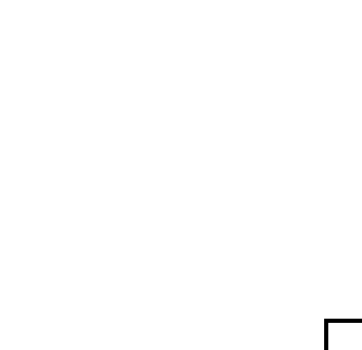
\includegraphics[width=12cm]{figures/section6-module-m/UserInputInformation.pdf}
    \caption{UserInputInformation}
    \label{fig:UserInputInformation}
\end{figure}

% M1-2-1
\subsubsection{UserLogoutScreen}
\begin{figure}[H]
    \centering
    \includegraphics[width=12cm]{figures/section6_user_defmodule_front/section6_UserLogoutScreen.pdf}
    \caption{UserLogoutScreen}
    \label{fig:UserLogoutScreen}
\end{figure}

% M1-2-2
\subsubsection{UserLogout}
\begin{figure}[H]
    \centering
    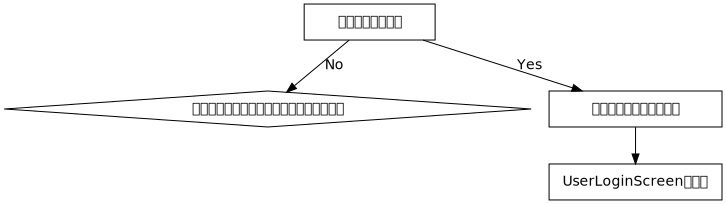
\includegraphics[width=12cm]{figures/section6-module-m/UserLogout.pdf}
    \caption{UserLogout}
    \label{fig:UserLogout}
\end{figure}

% M1-3-1
\subsubsection{UserDeleteScreen}
\begin{figure}[H]
    \centering
    \includegraphics[width=12cm]{figures/section6_user_defmodule_front/section6_UserDeleteScreen.pdf}
    \caption{UserDeleteScreen}
    \label{fig:UserDeleteScreen}
\end{figure}

% M1-3-2
\subsubsection{UserDeleteInformation}
\begin{figure}[H]
    \centering
    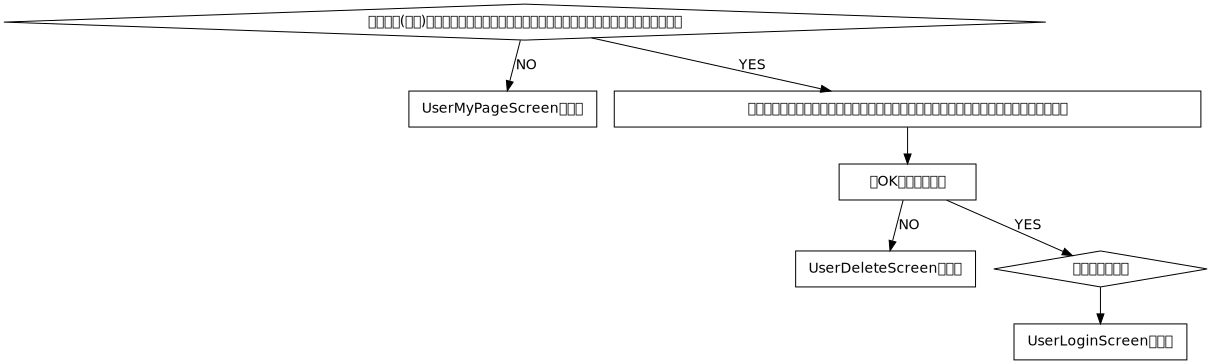
\includegraphics[width=12cm]{figures/section6-module-m/UserDeleteInformation.pdf}
    \caption{UserDeleteInformation}
    \label{fig:UserDeleteInformation}
\end{figure}

% M1-4-1
\subsubsection{UserContactScreen}
\begin{figure}[H]
    \centering
    \includegraphics[width=12cm]{figures/section6_user_defmodule_front/section6_UserContactScreen.pdf}
    \caption{UserContactScreen}
    \label{fig:UserContactScreen}
\end{figure}

% M1-4-2
\subsubsection{UserInputContactInformation}
\begin{figure}[H]
    \centering
    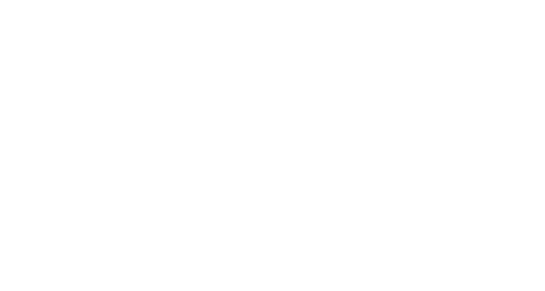
\includegraphics[width=12cm]{figures/section6-module-m/UserInputContactInformation.pdf}
    \caption{UserInputContactInformation}
    \label{fig:UserInputContactInformation}
\end{figure}

% M1-5-1
\subsubsection{UserGetPostNumber}
\begin{figure}[H]
    \centering
    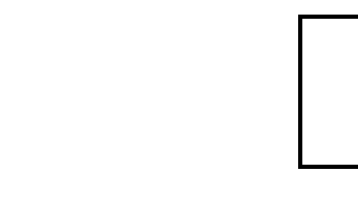
\includegraphics[width=12cm]{figures/section6-module-m/UserGetPostNumber.pdf}
    \caption{UserGetPostNumber}
    \label{fig:UserGetPostNumber}
\end{figure}

% M1-5-2
\subsubsection{UserMapViewScreen}
\begin{figure}[H]
    \centering
    \includegraphics[width=12cm]{figures/section6_user_defmodule_front/section6_UserMapViewScreen.pdf}
    \caption{UserMapViewScreen}
    \label{fig:UserMapViewScreen}
\end{figure}

% M1-6-1
\subsubsection{UserGetPinDetail}
\begin{figure}[H]
    \centering
    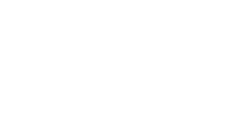
\includegraphics[width=12cm]{figures/section6-module-m/UserGetPinDetail.pdf}
    \caption{UserGetPinDetail}
    \label{fig:UserGetPinDetail}
\end{figure}

% M1-6-2,1-7-1,2
\subsubsection{UserPinDetailScreen}
\begin{figure}[H]
    \centering
    \includegraphics[width=12cm]{figures/section6_user_defmodule_front/section6_UserPinDetailScreen.pdf}
    \caption{UserPinDetailScreen}
    \label{fig:UserPinDetailScreen}
\end{figure}

\subsubsection{UserPinPostScreen}
\begin{figure}[H]
    \centering
    \includegraphics[width=12cm]{figures/section6_user_defmodule_front/section6_UserPinPostScreen.pdf}
    \caption{UserPinPostScreen}
    \label{fig:UserPinPostScreen}
\end{figure}

\subsubsection{UserGetLocation}
\begin{figure}[H]
    \centering
    \includegraphics[width=12cm]{figures/section6_user_defmodule_front/section6_UserGetLocation.pdf}
    \caption{UserGetLocation}
    \label{fig:UserGetLocation}
\end{figure}

% M1-7-3
\subsubsection{UserNameSearch}
\begin{figure}[H]
    \centering
    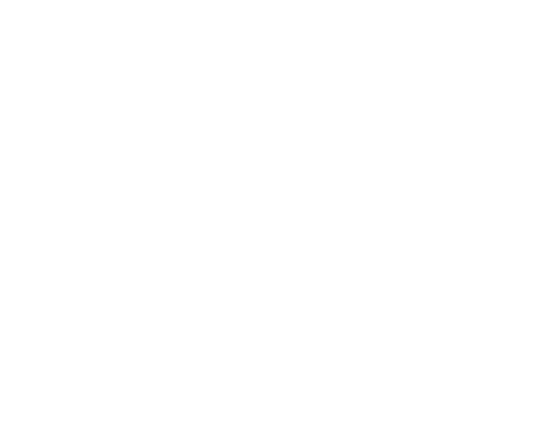
\includegraphics[width=12cm]{figures/section6-module-m/UserNameSearch.pdf}
    \caption{UserNameSearch}
    \label{fig:UserNameSearch}
\end{figure}

% M1-7-4
\subsubsection{UserGetDate}
\begin{figure}[H]
    \centering
    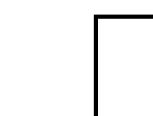
\includegraphics[width=12cm]{figures/section6-module-m/UserGetDate.pdf}
    \caption{UserGetDate}
    \label{fig:UserGetDate}
\end{figure}

% M1-7-5
\subsubsection{UserInputPinDetail}
\begin{figure}[H]
    \centering
    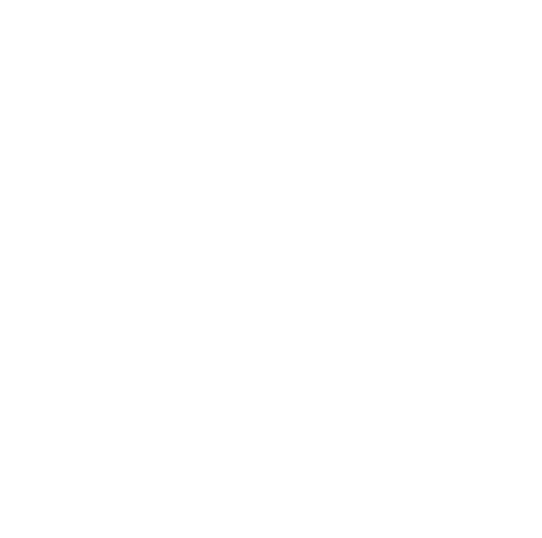
\includegraphics[width=12cm]{figures/section6-module-m/UserInputPinDetail.pdf}
    \caption{UserInputPinDetail}
    \label{fig:UserInputPinDetail}
\end{figure}

% M1-8~M1-15-1
\subsubsection{KeywordSearch}
\begin{figure}[H]
    \centering
    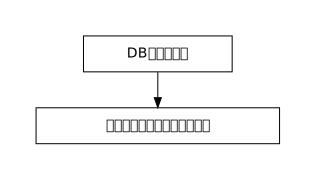
\includegraphics[width=12cm]{figures/section6-module-m/KeywordSearch.pdf}
    \caption{KeywordSearch}
    \label{fig:KeywordSearch}
\end{figure}

\subsubsection{GenreSearch}
\begin{figure}[H]
    \centering
    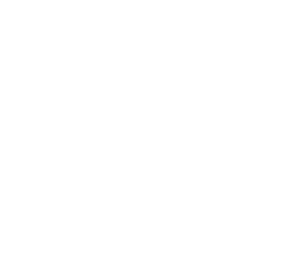
\includegraphics[width=12cm]{figures/section6-module-m/GenreSearch.pdf}
    \caption{GenreSearch}
    \label{fig:GenreSearch}
\end{figure}

\subsubsection{DateSearch }
\begin{figure}[H]
    \centering
    \includegraphics[width=12cm]{figures/section6-module-m/DataSearch.pdf}
    \caption{DateSearch }
    \label{fig:DateSearch }
\end{figure}

\subsubsection{SortDate}
\begin{figure}[H]
    \centering
    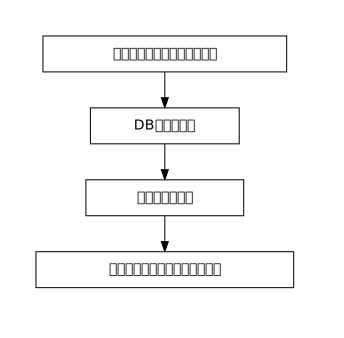
\includegraphics[width=12cm]{figures/section6-module-m/SortDate.pdf}
    \caption{SortDate}
    \label{fig:SortDate}
\end{figure}

\subsubsection{SortReaction}
\begin{figure}[H]
    \centering
    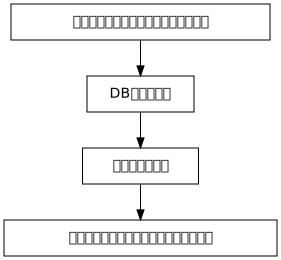
\includegraphics[width=12cm]{figures/section6-module-m/SortReaction.pdf}
    \caption{SortReaction}
    \label{fig:SortReaction}
\end{figure}

\subsubsection{SortDistance}
\begin{figure}[H]
    \centering
    \includegraphics[width=12cm]{figures/section6-module-m/SortDistance.pdf}
    \caption{SortDistance}
    \label{fig:SortDistance}
\end{figure}

\subsubsection{UserInputBlockInformation}
\begin{figure}[H]
    \centering
    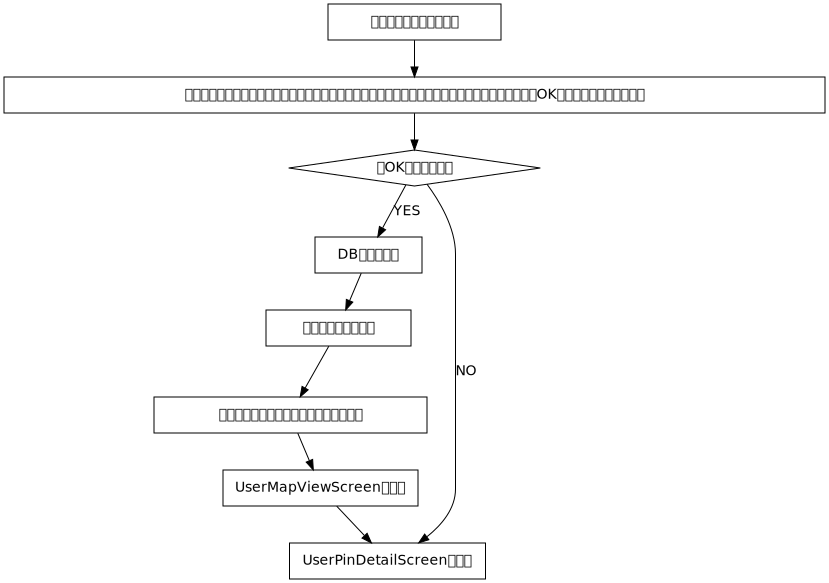
\includegraphics[width=12cm]{figures/section6-module-m/UserInputBlockInformation.pdf}
    \caption{UserInputBlockInformation}
    \label{fig:UserInputBlockInformation}
\end{figure}

\subsubsection{UserDeleteBlockInformation}
\begin{figure}[H]
    \centering
    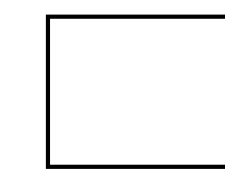
\includegraphics[width=12cm]{figures/section6-module-m/UserDeleteBlockInformation.pdf}
    \caption{UserDeleteBlockInformation}
    \label{fig:UserDeleteBlockInformation}
\end{figure}

% M1-15-2,1-16-1
\subsubsection{UserDeleteBlockScreen}
\begin{figure}[H]
    \centering
    \includegraphics[width=12cm]{figures/section6_user_defmodule_front/section6_UserDeleteBlockScreen.pdf}
    \caption{UserDeleteBlockScreen}
    \label{fig:UserDeleteBlockScreen}
\end{figure}

\subsubsection{UserReportScreen}
\begin{figure}[H]
    \centering
    \includegraphics[width=12cm]{figures/section6_user_defmodule_front/section6_UserReportScreen.pdf}
    \caption{UserReportScreen}
    \label{fig:UserReportScreen}
\end{figure}

% M1-16-2,M1-17-1
\subsubsection{UserInputReportInformation}
\begin{figure}[H]
    \centering
    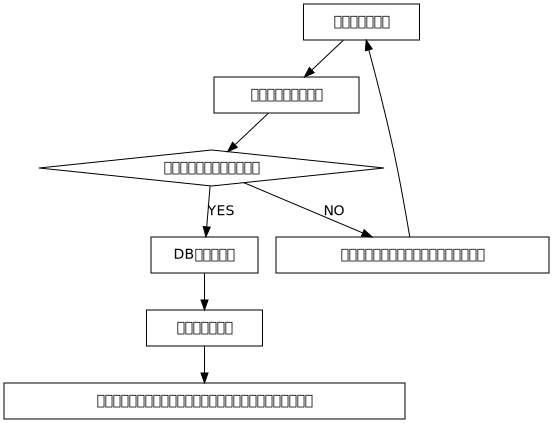
\includegraphics[width=12cm]{figures/section6-module-m/UserInputReportInformation.pdf}
    \caption{UserInputReportInformation}
    \label{fig:UserInputReportInformation}
\end{figure}

\subsubsection{UserDeletePinDetail }
\begin{figure}[H]
    \centering
    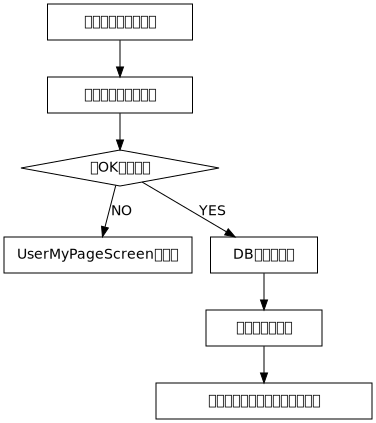
\includegraphics[width=12cm]{figures/section6-module-m/UserDeletePinDetail.pdf}
    \caption{UserDeletePinDetail }
    \label{fig:UserDeletePinDetail }
\end{figure}

% M1-17-2
\subsubsection{UserDeletePinScreen}
\begin{figure}[H]
    \centering
    \includegraphics[width=12cm]{figures/section6_user_defmodule_front/section6_UserDeletePinScreen.pdf}
    \caption{UserDeletePinScreen}
    \label{fig:UserDeletePinScreen}
\end{figure}

% M1-18-1
\subsubsection{UserInputReactionInformation}
\begin{figure}[H]
    \centering
    \includegraphics[scale=0.6]{figures/section6_module_iwamura/M1-18-1.pdf}
    \caption{UserInputReactionInformation}
    \label{fig:UserInputReactionInformation}
\end{figure}

% M1-18-2
\subsubsection{UserReactionScreen}
\begin{figure}[H]
    \centering
    \includegraphics[width=12cm]{figures/section6_user_defmodule_front/section6_UserReactionScreen.pdf}
    \caption{UserReactionScreen}
    \label{fig:UserReactionScreen}
\end{figure}

% M1-19, M1-20
\subsubsection{UserGetReactionList}
\begin{figure}[H]
    \centering
    \includegraphics[scale=0.6]{figures/section6_module_iwamura/M1-19.pdf}
    \caption{UserGetReactionList}
    \label{fig:UserGetReactionList}
\end{figure}

\subsubsection{InputBusinessRequestInformation}
\begin{figure}[H]
    \centering
    \includegraphics[scale=0.6]{figures/section6_module_iwamura/M1-20.pdf}
    \caption{InputBusinessRequestInformation}
    \label{fig:InputBusinessRequestInformation}
\end{figure}

% M1-21
\subsubsection{UserMyPageScreen}
\begin{figure}[H]
    \centering
    \includegraphics[width=12cm]{figures/section6_user_defmodule_front/section6_UserMyPageScreen.pdf}
    \caption{UserMyPageScreen}
    \label{fig:UserMyPageScreen}
\end{figure}

% 事業者側モジュール
\subsection{事業者側モジュール}
% モジュール間遷移図
\subsubsection{事業者会員モジュール間遷移図}
事業者会員モジュールとして,モジュール間遷移図を図\ref{fig:bus_moduletrans}に示す.
\begin{figure}[H]
    \centering
    \includesvg[inkscapelatex=false, width=0.8\linewidth]{./figures/section6_businessmodule.svg}
    \caption{モジュール間遷移図}
    \label{fig:bus_moduletrans}
\end{figure}

\subsubsection{BusinessInputInformation}
\begin{figure}[H]
    \centering
    \includegraphics[scale=0.6]{figures/section6_business_module/M3-1.pdf}
    \caption{BusinessInputInformation}
    \label{fig:BusinessInputInformation}
\end{figure}

\subsubsection{BusinessSelectMyPage}
\begin{figure}[H]
    \centering
    \includegraphics[scale=0.6]{figures/section6_business_module/M3-2-1.pdf}
    \caption{BusinessSelectMyPage}
    \label{fig:BusinessSelectMyPage}
\end{figure}

\subsubsection{}



\if0
\begin{figure}[H]
    \centering
    \includegraphics[scale=0.6]
    \caption{}
    \label{fig:}
\end{figure}
\fi

% 管理者側モジュール
\subsection{管理者側モジュール}
% モジュール間遷移図
\subsubsection{管理者モジュール間遷移図}
管理者モジュールとして,モジュール間遷移図を図\ref{fig:admin_moduletrans}に示す.
\begin{figure}[H]
    \centering
    \includesvg[inkscapelatex=false, width=0.8\linewidth]{./figures/section6_adminmodule.svg}
    \caption{モジュール間遷移図}
    \label{fig:admin_moduletrans}
\end{figure}

% M3-1-1
\subsubsection{AdminLoginScreen}
\begin{figure}[H]
    \centering
    \includegraphics[width=12cm]{./figures/section6_admin_defmodule_front/section6_AdminLoginScreen.pdf}
    \caption{AdminLoginScreen}
    \label{fig:AdminLoginScreen}
\end{figure}
% M3-1-2
\subsubsection{AdminInputInformation}
\begin{figure}[H]
    \centering
    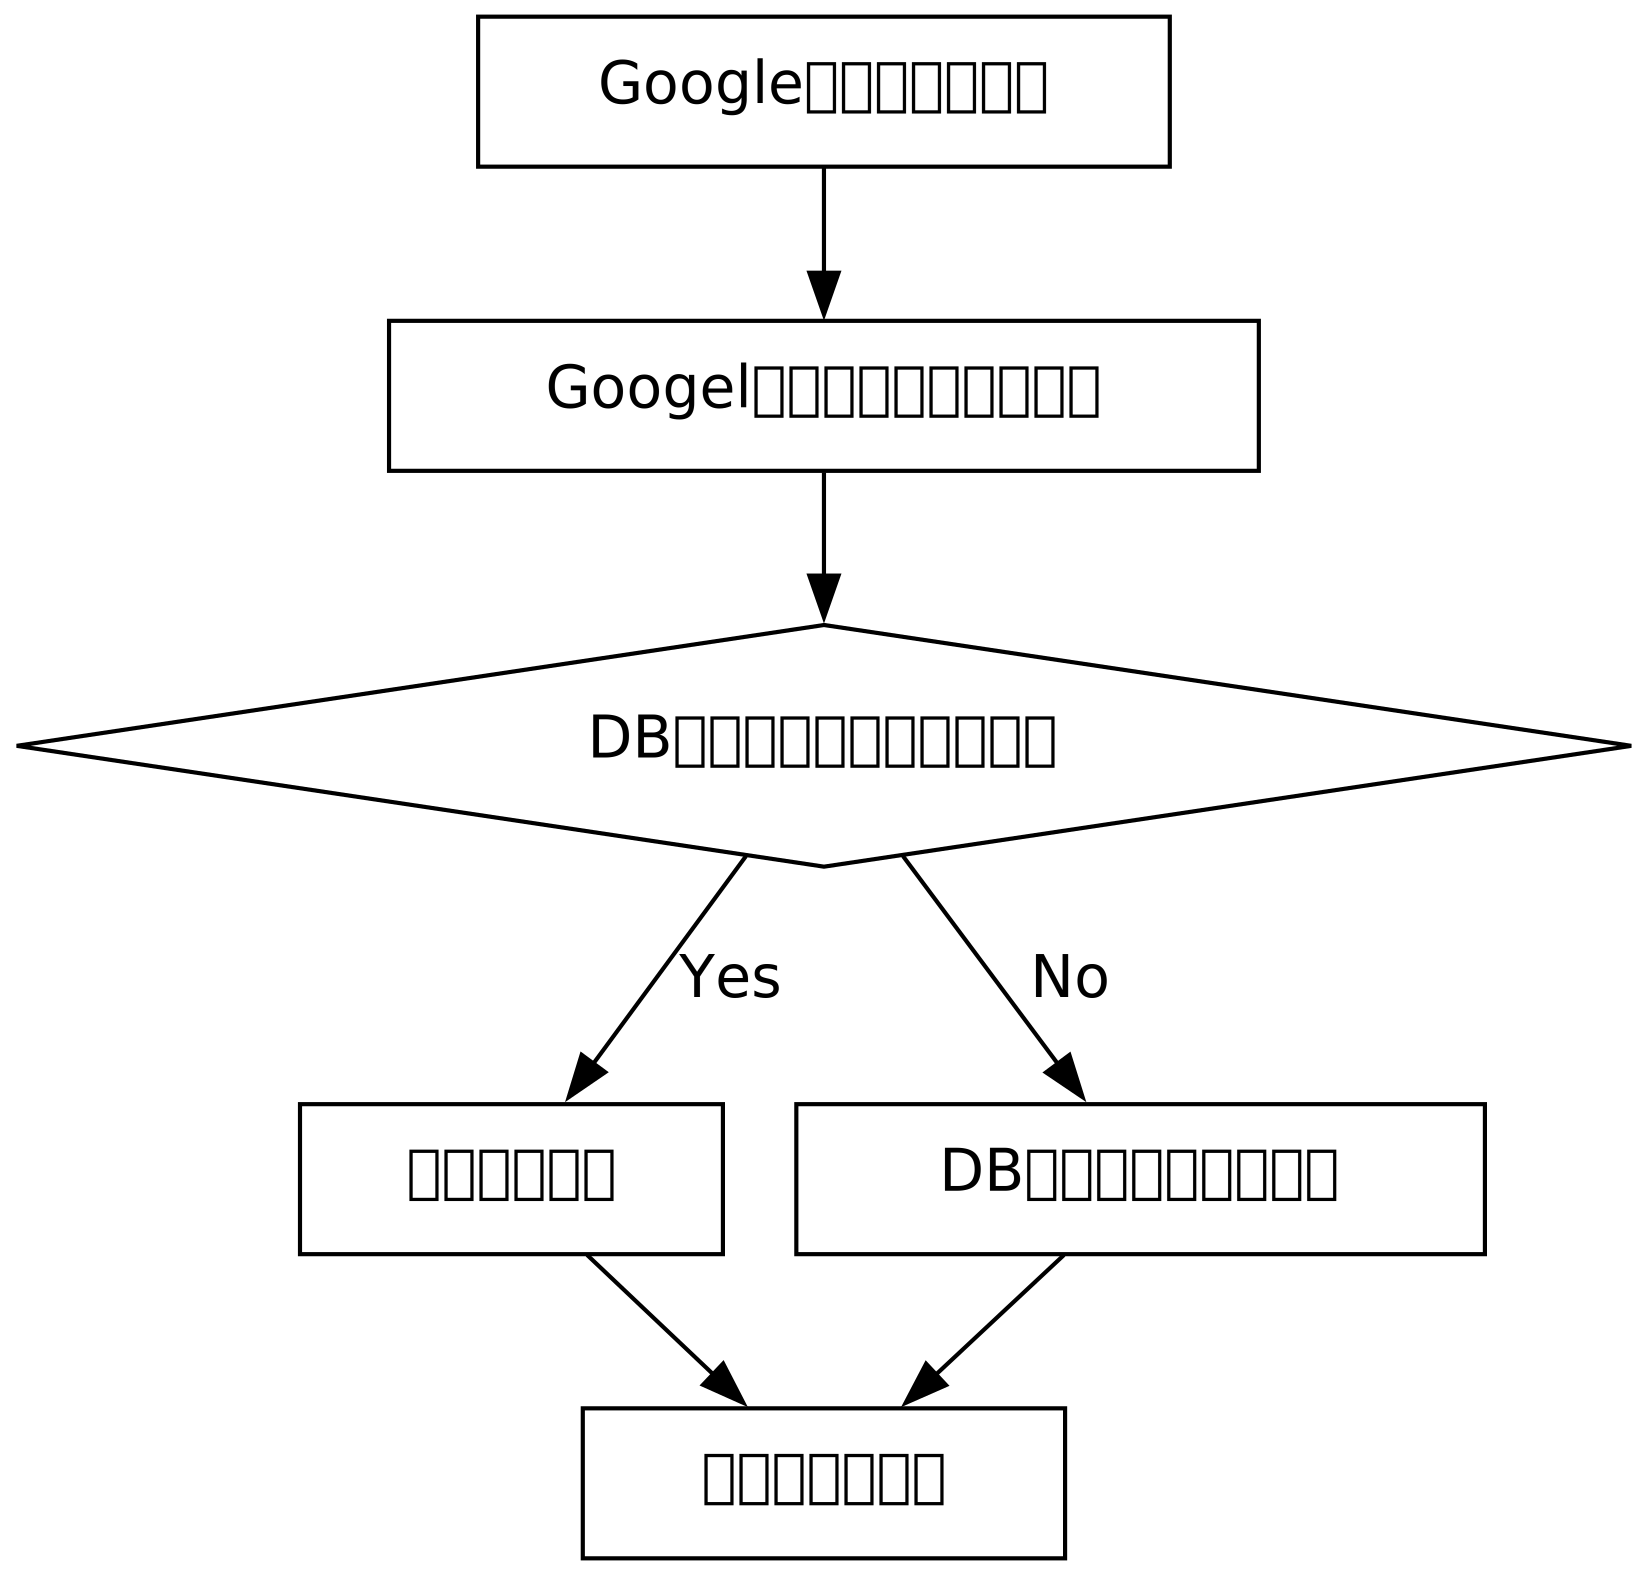
\includegraphics[keepaspectratio, width=0.8\linewidth]{figures/sato/AdminInputInformation.pdf}
    \caption{AdminInputInformation}
    \label{fig:AdminInputInformation}
\end{figure}

% M3-2
\subsubsection{AdminLogout}
\begin{figure}[H]
    \centering
    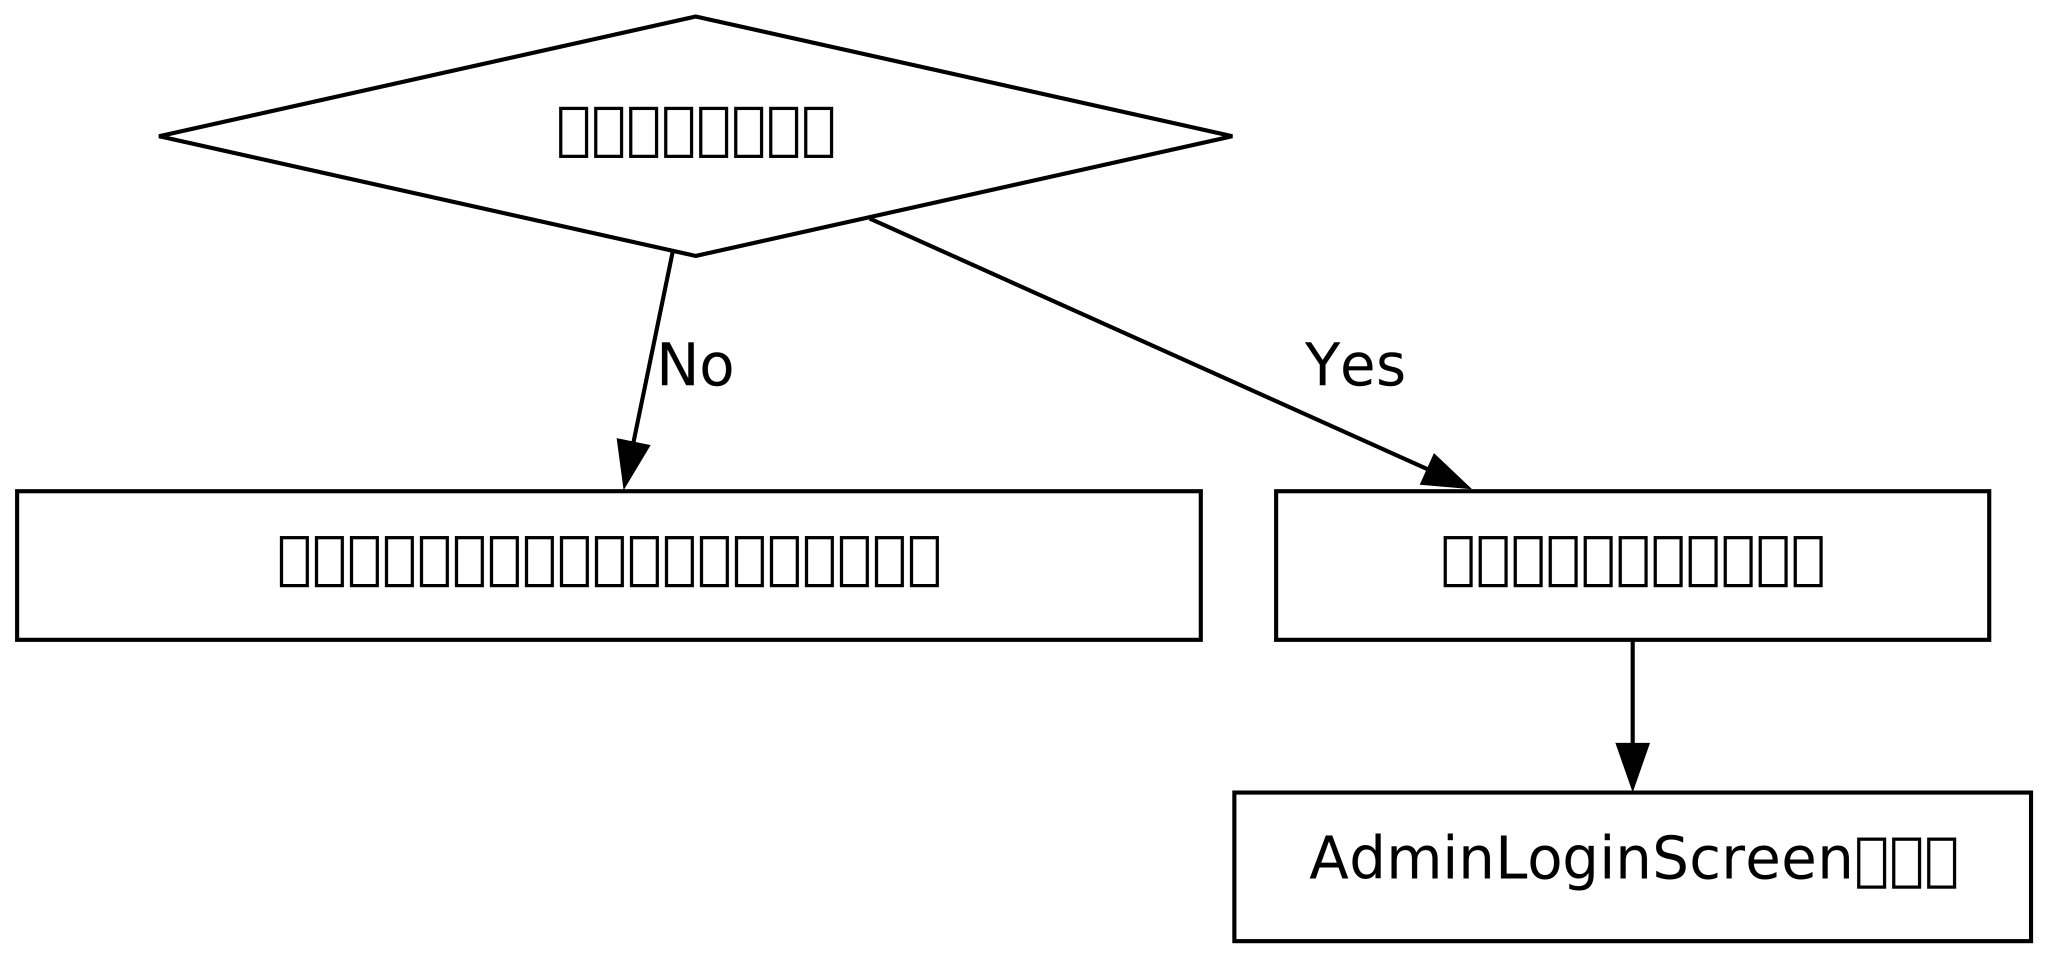
\includegraphics[keepaspectratio, width=0.8\linewidth]{figures/sato/AdminLogout.pdf}
    \caption{AdminLogout}
    \label{fig:AdminLogout}
\end{figure}

% M3-3-1
\subsubsection{AdminGetTotalUserNumber}
\begin{figure}[H]
    \centering
    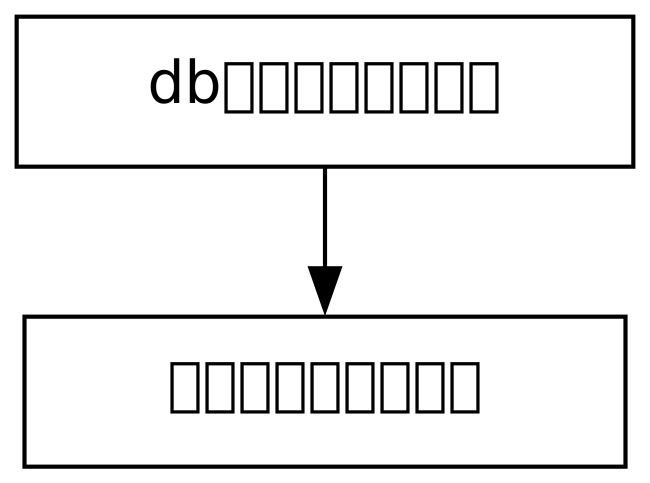
\includegraphics[keepaspectratio, width=0.8\linewidth]{figures/sato/AdminGetTotalUserNumber.pdf}
    \caption{AdminGetTotalUserNumber}
    \label{fig:AdminGetTotalUserNumber}
\end{figure}
% M3-3-2
\subsubsection{AdminGetActiveUserNumber}
\begin{figure}[H]
    \centering
    \includegraphics[keepaspectratio, width=0.8\linewidth]{figures/sato/AdminGetActiveUserNumber.pdf}
    \caption{AdminGetActiveUserNumber}
    \label{fig:AdminGetActiveUserNumber}
\end{figure}
% M3-3-3
\subsubsection{AdminGetTotalPostNumber}
\begin{figure}[H]
    \centering
    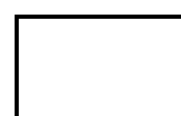
\includegraphics[keepaspectratio, width=0.8\linewidth]{figures/sato/AdminGetTotalPostNumber.pdf}
    \caption{AdminGetTotalPostNumber}
    \label{fig:AdminGetTotalPostNumber}
\end{figure}
% M3-3-4
\subsubsection{AdminGetTotalReactionNumber}
\begin{figure}[H]
    \centering
    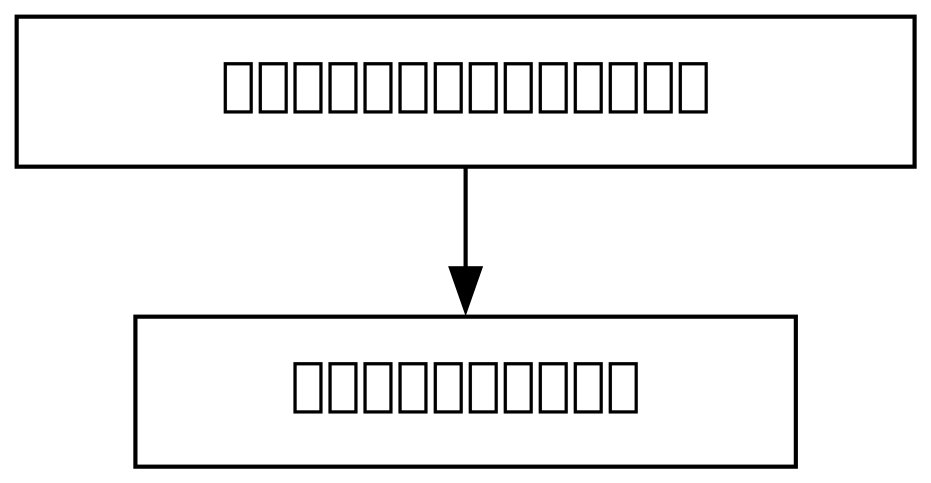
\includegraphics[keepaspectratio, width=0.8\linewidth]{figures/sato/AdminGetTotalReactionNumber.pdf}
    \caption{AdminGetTotalReactionNumber}
    \label{fig:AdminGetTotalReactionNumber}
\end{figure}
% M3-3-5
\subsubsection{AdminGetBusinessAccountNumber}
\begin{figure}[H]
    \centering
    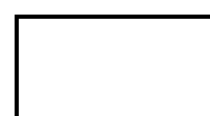
\includegraphics[keepaspectratio, width=0.8\linewidth]{figures/sato/AdminGetBusinessAccountNumber.pdf}
    \caption{AdminGetBusinessAccountNumber}
    \label{fig:AdminGetBusinessAccountNumber}
\end{figure}
% M3-3-6
\subsubsection{AdminGetNotReportNumber}
\begin{figure}[H]
    \centering
    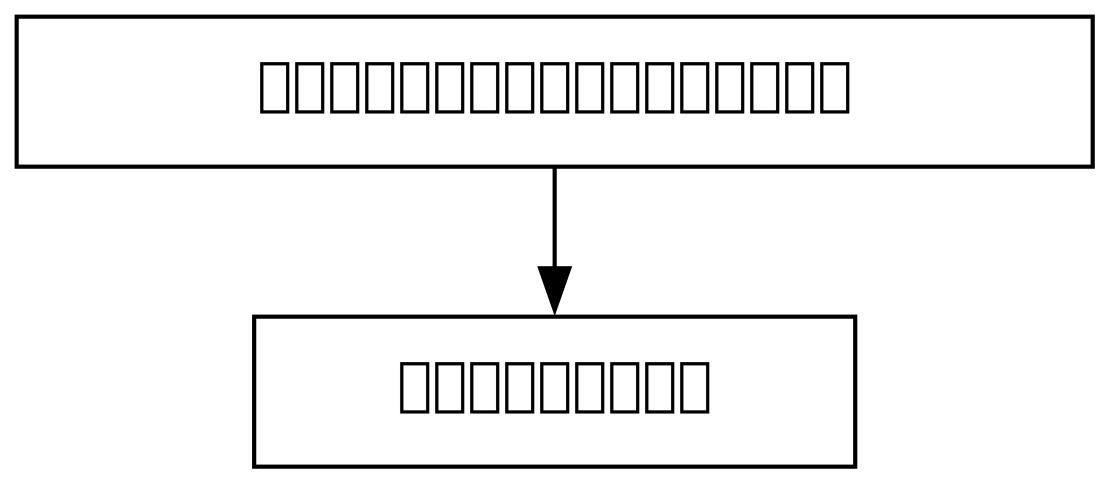
\includegraphics[keepaspectratio, width=0.8\linewidth]{figures/sato/AdminGetNotReportNumber.pdf}
    \caption{AdminGetNotReportNumber}
    \label{fig:AdminGetNotReportNumber}
\end{figure}


% M3-3-7,8
\subsubsection{AdminDashboardScreen}
\begin{figure}[H]
    \centering
    \includegraphics[width=7cm]{./figures/section6_admin_defmodule_front/section6_AdminDashboardScreen.pdf}
    \caption{AdminDashboardScreen}
    \label{fig:AdminDashboardScreen}
\end{figure}

\subsubsection{AdminDashboardGraphScreen}
\begin{figure}[H]
    \centering
    \includegraphics[width=7cm]{./figures/section6_admin_defmodule_front/section6_AdminDashboardGraphScreen.pdf}
    \caption{AdminDashboardGraphScreen}
    \label{fig:AAdminDashboardGraphScreen}
\end{figure}

% M3-4-1
\subsubsection{ProcessReportDeletePinDetail}
\begin{figure}[H]
    \centering
    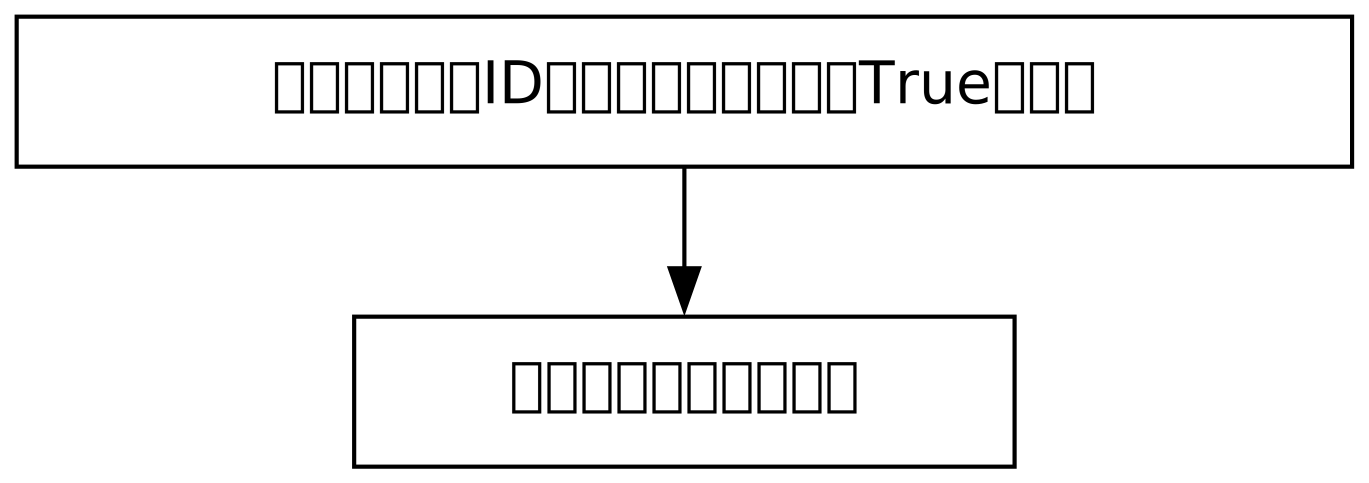
\includegraphics[keepaspectratio, width=0.8\linewidth]{figures/sato/ProcessReportDeletePinDetail.pdf}
    \caption{ProcessReportDeletePinDetail}
    \label{fig:ProcessReportDeletePinDetail}
\end{figure}
% M3-4-2
\subsubsection{ProcessReportScreen}
\begin{figure}[H]
    \centering
    \includegraphics[width=12cm]{./figures/section6_admin_defmodule_front/section6_ProcessReportScreen.pdf}
    \caption{ProcessReportScreen}
    \label{fig:ProcessReportScreen}
\end{figure}
% M3-5-1
\subsubsection{InputBusinessInformation}
\begin{figure}[H]
    \centering
    \includegraphics[keepaspectratio, width=0.8\linewidth]{figures/sato/InputBusinessInformation.pdf}
    \caption{InputBusinessInformation}
    \label{fig:InputBusinessInformation}
\end{figure}
% M3-5-2
\subsubsection{ProcessBusinessRequestScreen}
\begin{figure}[H]
    \centering
    \includegraphics[width=7cm]{./figures/section6_admin_defmodule_front/section6_ProcessBusinessRequestScreen.pdf}
    \caption{ProcessBusinessRequestScreen}
    \label{fig:ProcessBusinessRequestScreen}
\end{figure}

% M3-6-1
\subsubsection{AdminDeleletePost}
\begin{figure}[H]
    \centering
    \includegraphics[keepaspectratio, width=0.8\linewidth]{figures/sato/AdminDeleletePost.pdf}
    \caption{AdminDeleletePost}
    \label{fig:AdminDeleletePost}
\end{figure}
% M3-6-2
\subsubsection{SendUserMessage}
\begin{figure}[H]
    \centering
    \includegraphics[keepaspectratio, width=0.8\linewidth]{figures/sato/SendUserMessage.pdf}
    \caption{SendUserMessage}
    \label{fig:SendUserMessage}
\end{figure}

% M3-7
\subsubsection{AdminDeleteAccount}
\begin{figure}[H]
    \centering
    \includegraphics[keepaspectratio, width=0.8\linewidth]{figures/sato/AdminDeleteAccount.pdf}
    \caption{AdminDeleteAccount}
    \label{fig:AdminDeleteAccount}
\end{figure}
% M3-8-1
\subsubsection{ProcessContact}
\begin{figure}[H]
    \centering
    \includegraphics[keepaspectratio, width=0.8\linewidth]{figures/sato/ProcessContact.pdf}
    \caption{ProcessContact}
    \label{fig:ProcessContact}
\end{figure}
% M3-8-2
\subsubsection{SendUserMailContact}
\begin{figure}[H]
    \centering
    \includegraphics[keepaspectratio, width=0.8\linewidth]{figures/sato/SendUserMailContact.pdf}
    \caption{SendUserMailContact}
    \label{fig:SendUserMailContact}
\end{figure}
% M3-8-3
\subsubsection{ProcessContactScreen}
\begin{figure}[H]
    \centering
    \includegraphics[width=12cm]{./figures/section6_admin_defmodule_front/section6_ProcessContactScreen.pdf}
    \caption{AdminLoginScreen}
    \label{fig:ProcessContactScreen}
\end{figure}

% データベース設計
\section{データベース設計}
\subsection{ER図}
本データベースのER図を図 \ref{fig:sec7er} に示す.

\begin{figure}[H]
    \centering
    \includesvg[inkscapelatex=false, width=0.8\linewidth]{figures/section7_database.svg}
    \caption{ER図}
    \label{fig:sec7er}
\end{figure}

\subsection{テーブル一覧}
本システムのデータベースのテーブルを表 \ref{tb:user} から表 \ref{tb:reaction} 示す.

\begin{table}[H]
    \centering
    \caption{会員情報}
    \label{tb:user}
    \begin{tabular}{|c|c|c|c|c|c|} \hline
        カラム名 & PK & FK & その他の制約 & 論理データ型 & 説明 \\ \hline\hline
        id & ○ & & not null & VARCHAR(50) & Google ID \\ \hline
        gmail & & & not null & VARCHAR(100) & メールアドレス \\ \hline
        role & & & not null & ENUM('user','business','admin') & 会員区分 \\ \hline
        registrationDate & & & not null & DATETIME & 登録日 \\ \hline
    \end{tabular}
\end{table}

\begin{table}[H]
    \centering
    \caption{セッション情報}
    \label{tb:session}
    \begin{tabular}{|c|c|c|c|c|c|} \hline
        カラム名 & PK & FK & その他の制約 & 論理データ型 & 説明 \\ \hline\hline
        sessionId & ○ & & not null & VARCHAR(255) & セッションID \\ \hline
        googleId & & ○ & not null & VARCHAR(50) & Google ID \\ \hline
        expiry & & & not null & DATETIME & 有効期限 \\ \hline
    \end{tabular}
\end{table}

\begin{table}[H]
    \centering
    \caption{事業者会員情報}
    \label{tb:business}
    \begin{tabular}{|c|c|c|c|c|c|} \hline
        カラム名 & PK & FK & その他の制約 & 論理データ型 & 説明 \\ \hline\hline
        id & ○ & & not null & INT & ID \\ \hline
        businessName & & & not null & VARCHAR(50) & 事業者名 \\ \hline
        kanaBusinessName & & & not null & VARCHAR(50) & カナ事業者名 \\ \hline
        zipCode & & & not null & INT & 郵便番号 \\ \hline
        address & & & not null & VARCHAR(100) & 住所 \\ \hline
        phone & & & not null & INT & 電話番号 \\ \hline
        registDate & & & not null & DATETIME & 登録日時 \\ \hline
        profileImage & & & & BLOB & プロフィール画像 \\ \hline
        userId & & ○ & not null & VARCHAR(50) & Google ID \\ \hline
        placeId & & ○ & not null & INT & 場所ID \\ \hline
    \end{tabular}
\end{table}

\begin{table}[H]
    \centering
    \caption{ブロック情報}
    \label{tb:block}
    \begin{tabular}{|c|c|c|c|c|c|} \hline
        カラム名 & PK & FK & その他の制約 & 論理データ型 & 説明 \\ \hline\hline
        id & ○ & & not null & INT & ID \\ \hline
        blockerId & & ○ & not null & VARCHAR(50) & ブロックしたユーザーのGoogle ID \\ \hline
        blockedId & & ○ & not null & VARCHAR(50) & ブロックされたユーザーのGoogle ID \\ \hline
    \end{tabular}
\end{table}

\begin{table}[H]
    \centering
    \caption{問い合わせ情報}
    \label{tb:ask}
    \begin{tabular}{|c|c|c|c|c|c|} \hline
        カラム名 & PK & FK & その他の制約 & 論理データ型 & 説明 \\ \hline\hline
        id & ○ & & not null & INT & ID \\ \hline
        date & & & not null & DATETIME & 問い合わせ日時 \\ \hline
        subject & & & not null & VARCHAR(100) & 件名 \\ \hline
        text & & & not null & TEXT & 本文 \\ \hline
        askId & & ○ & not null & VARCHAR(50) & 問い合わせたユーザーのGoogle ID \\ \hline
        askFlag & & & not null & BOOLEAN & 問い合わせフラグ \\ \hline
    \end{tabular}
\end{table}

\begin{table}[H]
    \centering
    \caption{投稿内容}
    \label{tb:post}
    \begin{tabular}{|c|c|c|c|c|c|} \hline
        カラム名 & PK & FK & その他の制約 & 論理データ型 & 説明 \\ \hline\hline
        id & ○ & & not null & INT & ID \\ \hline
        placeId & & ○ & not null & INT & 場所ID \\ \hline
        userId & & ○ & not null & VARCHAR(50) & 投稿者ID \\ \hline
        postDate & & & not null & DATETIME & 投稿日時 \\ \hline
        title & & & not null & VARCHAR(50) & 投稿のタイトル \\ \hline
        text & & & not null & TEXT & 投稿の説明文 \\ \hline
        postImage & & & & BLOB & 投稿画像 \\ \hline
        numReaction & & & not null & INT & リアクション数 \\ \hline
        numView & & & not null & INT & 閲覧数 \\ \hline
        genreId & & ○ & not null & INT & ジャンルID \\ \hline
    \end{tabular}
\end{table}

\begin{table}[H]
    \centering
    \caption{場所情報}
    \label{tb:place}
    \begin{tabular}{|c|c|c|c|c|c|} \hline
        カラム名 & PK & FK & その他の制約 & 論理データ型 & 説明 \\ \hline\hline
        placeId & ○ & & not null & INT & 場所ID \\ \hline
        numPost & & & not null & INT & 投稿数 \\ \hline
        latitude & & & not null & DOUBLE & 緯度 \\ \hline
        longitude & & & not null & DOUBLE & 経度 \\ \hline
    \end{tabular}
\end{table}

\begin{table}[H]
    \centering
    \caption{ジャンル情報}
    \label{tb:genre}
    \begin{tabular}{|c|c|c|c|c|c|} \hline
        カラム名 & PK & FK & その他の制約 & 論理データ型 & 説明 \\ \hline\hline
        genreId & ○ & & not null & INT & ジャンルID \\ \hline
        genreName & & & not null & 
        \begin{tabular}{c}
            ENUM('food', 'event', 'scene', \\'store', 'emergency', 'other')
        \end{tabular}
        & ジャンル名 \\ \hline
        color & & & not null & VARCHAR(6) & 表示色 \\ \hline
    \end{tabular}
\end{table}

\begin{table}[H]
    \centering
    \caption{通報情報}
    \label{tb:report}
    \begin{tabular}{|c|c|c|c|c|c|} \hline
        カラム名 & PK & FK & その他の制約 & 論理データ型 & 説明 \\ \hline\hline
        id & ○ & & not null & INT & ID \\ \hline
        userId & & ○ & not null & VARCHAR(50) & 通報したユーザーのGoogle ID \\ \hline
        postId & & ○ & not null & INT & 対象投稿ID \\ \hline
        reason & & & not null & TEXT & 通報理由 \\ \hline
        date & & & not null & DATETIME & 通報日時 \\ \hline
        reportFlag & & & not null & BOOLEAN & 対応済みフラグ \\ \hline
        removeFlag & & & not null & BOOLEAN & 削除フラグ \\ \hline
    \end{tabular}
\end{table}

\begin{table}[H]
    \centering
    \caption{事業者申請情報}
    \label{tb:businessReq}
    \begin{tabular}{|c|c|c|c|c|c|} \hline
        カラム名 & PK & FK & その他の制約 & 論理データ型 & 説明 \\ \hline\hline
        id & ○ & & not null & INT & ID \\ \hline
        name & & & not null & VARCHAR(50) & 事業者名 \\ \hline
        address & & & not null & VARCHAR(100) & 住所 \\ \hline
        phone & & & not null & INT & 電話番号 \\ \hline
        userId & & ○ & not null & VARCHAR(50) & 申請者のGoogle ID \\ \hline
    \end{tabular}
\end{table}

\begin{table}[H]
    \centering
    \caption{リアクション情報}
    \label{tb:reaction}
    \begin{tabular}{|c|c|c|c|c|c|} \hline
        カラム名 & PK & FK & その他の制約 & 論理データ型 & 説明 \\ \hline\hline
        id & ○ & & not null & INT & ID \\ \hline
        userId & ○ & ○ & not null & VARCHAR(50) & リアクションをしたユーザーのGoogle ID \\ \hline
        postId & & ○ & not null & INT & 投稿ID \\ \hline
    \end{tabular}
\end{table}
\end{document}
